%% ============================================================================
%% AP-PEN --- arXiv preprint draft
%% ACM acmart / sigconf, two-column, non-ACM author version.
%%
%% Built from the MSc thesis source (main(3).tex). Content is unchanged; the
%% following thesis-only apparatus has been removed because it does not belong
%% in a preprint:
%%   * UCL Individual Project cover sheet (\includepdf)
%%   * table of contents
%%   * the "All models are wrong" epigraph and the UCL logo plate
%%   * running heads naming the department, programme and academic year
%%   * the UCL page-budget / marking-guidance comment blocks
%%   * the Declaration of AI Use (Cat. 2) -- a UCL submission requirement
%%   * the two red draft markers (\todo and [TODO-FIX]); see the notes below
%% The nomenclature, which was thesis front matter, is retained as Appendix A.
%%
%% Compile: pdflatex -> bibtex -> pdflatex -> pdflatex
%% ============================================================================
\documentclass[sigconf, authorversion=true, nonacm=true]{acmart}

%% No ACM reference block, no conference/DOI footer: this is a preprint.
\settopmatter{printacmref=false}
\renewcommand\footnotetextcopyrightpermission[1]{}
\setcopyright{none}
\pagestyle{plain}

%% ── Packages ────────────────────────────────────────────────────────────────
%% acmart already provides amsmath, amssymb, amsthm, graphicx, xcolor, hyperref,
%% booktabs and libertine+newtxmath. Do NOT re-add geometry, caption, float,
%% fontenc, inputenc, setspace, fancyhdr, hyperref or cite -- acmart either
%% supplies them or refuses to compile alongside them.
\usepackage{mathtools}                      % \multlined, \coloneqq
\usepackage{subcaption}                     % subfigures: (a), (b), (c)
\usepackage{threeparttable}                 % table notes
\usepackage{multirow}
\usepackage{siunitx}
\usepackage{enumitem}
\usepackage{tikz}
\usetikzlibrary{positioning,arrows.meta,fit,backgrounds,calc}

%% Let a column end short rather than stretching its internal glue to reach the
%% bottom margin. Under the two-column default (\flushbottom) any shortfall is
%% absorbed by the most stretchable glue in the column -- which is the space
%% around a section heading -- producing a large gap above that heading instead
%% of a slightly short column. Delete this line to get \flushbottom back.
\raggedbottom

%% Two-column prose with long technical compounds needs a looser tolerance.
\tolerance=2000
\emergencystretch=3em
\allowdisplaybreaks

%% ── Custom math shortcuts for this project ──────────────────────────────────
\DeclareMathOperator{\E}{\mathbb{E}}        % Expectation
\newcommand{\R}{\mathbb{R}}                  % Real numbers
\newcommand{\bx}{\mathbf{x}}                % Bold x (input vector)
\newcommand{\btheta}{\boldsymbol{\theta}}    % Network parameters
\newcommand{\Lhat}{\widehat{\mathcal{L}}}   % WamOL loss
\newcommand{\convyield}{\delta}             % Convenience yield symbol
\newcommand{\meanrev}{\kappa}               % Mean-reversion speed
\newcommand{\longrun}{\alpha}               % Long-run convenience yield


\begin{document}

%% ── TOP MATTER ──────────────────────────────────────────────────────────────
\title[AP-PEN: Physics-Enforced Convenience-Yield Inversion]{AP-PEN: A Hard-Constrained,
Physics-Enforced Network for Convenience-Yield Inversion from Commodity Futures ---
A WamOL Approach}

\author{Evan Lynch}
\email{evan.lynch.25@ucl.ac.uk}
\affiliation{%
  \department{Department of Mechanical Engineering}
  \institution{University College London}
  \city{London}
  \country{United Kingdom}
}

\author{Lama Hamadeh}
%% TODO: confirm email and department before posting.
\email{l.hamadeh@ucl.ac.uk}
\affiliation{%
  \department{Department of Mechanical Engineering}
  \institution{University College London}
  \city{London}
  \country{United Kingdom}
}

\author{Carolyn E. Phelan}
\email{carolyn.phelan.14@ucl.ac.uk}
\affiliation{%
  \department{Department of Computer Science}
  \institution{University College London}
  \city{London}
  \country{United Kingdom}
}

\renewcommand{\shortauthors}{Lynch et al.}

\begin{abstract}
The convenience yield, the implied benefit of holding physical commodities, is a latent state inferred only from the term structure of futures prices. Traditional methods assume linear-Gaussian dynamics and never verify the recovered states against the governing PDE. We introduce AP-PEN, an Affine-Partitioned, Physics-Enforced Network, which inverts the two-factor Gibson--Schwartz model for the instantaneous convenience yield of WTI crude oil futures. Rather than penalising the system for breaching the governing PDE, AP-PEN imposes the model's affine coefficients analytically, so a single network need only parameterise the latent convenience yield path. The resulting architecture satisfies the PDE by design, leaving no residual loss to learn. Physics instead enters through a transition likelihood on the recovered path under the physical measure, alongside no-arbitrage and economic inequality constraints balanced by a gradient-norm scheme adapted from Hoshisashi et al.'s WamOL framework~\cite{Hoshisashi2024Whack-a-moleSurface}. Validated on simulated and real WTI data (2015--2026), AP-PEN's no-arbitrage variant uniquely avoids collapsing into implausible estimates during the April 2020 market dislocation, achieving three times lower error than the filter, but at the cost of degenerate structural parameters. On clean synthetic data, these constraints prove counterproductive, with the closed-form least squares estimate outperforming every network variant. This work extends WamOL and derivative-constrained PINNs to commodities, contributing an identifiability analysis and a hard-constrained estimator rather than a residual-based architecture.
\end{abstract}

\keywords{Physics-Enforced Neural Networks, Whack-a-mole Online Learning,
Convenience Yield, Gibson--Schwartz Model, Commodity Futures, Structural
Identifiability, No-Arbitrage Constraints}

\maketitle

\section{Introduction}
\label{sec:introduction}

Commodities such as crude oil are primarily traded via futures contracts: standardised agreements to buy or sell a fixed quantity of the underlying asset at a predetermined price on a set future date. These contracts allow speculators and hedgers to take positions on future price movements, and the resulting market activity makes futures prices a key mechanism for price discovery, aggregating participants' collective expectations of supply and demand. In crude oil markets specifically, the relationship between spot and futures prices is further shaped by the cost and benefit of physical storage, captured in the concept of convenience yield: the implicit return accruing to holders of the physical commodity rather than a futures contract. Estimating this variable is vital for risk management, hedging and procurement. This thesis focuses on WTI crude oil, the most widely benchmarked and liquid contract in the global oil market, as the setting for this estimation problem.

Accurate estimation in practice is difficult: convenience yield is, by nature, a \textit{latent} state and is not directly observable. Traditional approaches employ Kalman filters (KFs) to reconstitute and track hidden state variables in commodity pricing models~\cite{Schwartz1997TheHedging}. While highly useful, these assume linearity and Gaussian noise, ignoring the Partial Differential Equation (PDE) and no-arbitrage constraints inherent to the model.

Physics-informed neural networks (PINNs), an architecture within the broader unsupervised learning paradigm, are a comparatively recent development. While they have been widely applied across engineering and physics, embedding governing differential equations directly into the learning process, their adoption in financial computing has emerged only recently. Whack-a-mole Online Learning (WamOL) is one such example, integrating self-adaptive weights and online learning into the PINN framework. This thesis extends the work of Hoshisashi et al.~\cite{Hoshisashi2024Whack-a-moleSurface}, adapting WamOL to commodity markets to estimate the instantaneous convenience yield in the Gibson--Schwartz (GS) two-factor model. What carries over from WamOL is the gradient-norm loss balancer and the derivative-constrained inequality-penalty mechanism (\S\ref{sec:lit_pinns}); the PDE-residual loss term does not, since the exact affine imposition at the centre of AP-PEN (\S\ref{sec:pinn_inversion}) satisfies the pricing PDE by construction and leaves no residual to penalise.
This thesis therefore asks whether AP-PEN, a hard-constrained neural inversion of this kind, can recover convenience yield from observed futures term structure with comparable or superior accuracy to KF-based methods, while respecting the no-arbitrage structure of the GS PDE. Building on the GS PDE and its closed-form pricing equation, the aim of this thesis is to extend the WamOL framework to estimate the latent convenience yield in commodity markets using the GS two-factor model. The contributions and objectives of this thesis are as follows:

\begin{enumerate}[noitemsep]
    \item \textbf{Affine-partitioned latent-state inversion:} Separate the GS solution into analytical affine maps, $A(\tau)$ and $B(\tau)$, and a neural convenience-yield path, $\hat{\delta}_\phi(t)$, satisfying the pricing PDE by construction and replacing soft residual losses with hard structural constraints, transition likelihoods, and inequality penalties (\S\ref{sec:pinn_inversion}).
    \item \textbf{Identifiability analysis of the Gibson--Schwartz model:} Establish which risk-neutral parameters a futures panel can identify at all, so that the inversion is asked only for what the data can supply. We prove a futures panel determines only three parameter combinations $(\kappa, \sigma_2, m)$, where $m = \alpha^{\mathbb{Q}} + \rho\sigma_1\sigma_2/\kappa$; $\sigma_1$, $\rho$, and $\alpha^{\mathbb{Q}}$ are fundamentally unidentifiable from prices alone by any estimator (\S\ref{sec:identifiability}).
    \item \textbf{Commodity-specific economic constraints:} Formulate model-free inequality constraints tailored to physical markets, evaluated strictly on observations $(S_t, \tau, r_t)$ and the recovered path, avoiding model-based derivative constraints entirely, and measure whether they bind (\S\ref{sec:constraints}, \S\ref{sec:real_data}).
    \item \textbf{Validation on synthetic and real data:} Generate synthetic market data via Euler--Maruyama Monte Carlo simulation parameterised via Schwartz~\cite{Schwartz1997TheHedging} (\S\ref{sec:experimental_design}); validate against the ground-truth convenience yield on the synthetic dataset (\S\ref{sec:synthetic}); and apply the model to real Refinitiv WTI futures data, including out-of-sample pricing (\S\ref{sec:real_data}).
    \item \textbf{Kalman filter benchmarking:} Compare AP-PEN's predictions against a maximum-likelihood KF baseline fitted to the same WTI panel (\S\ref{sec:real_data}, \S\ref{sec:kalman}).
\end{enumerate}


% --- 1.3 Recent advances: PINNs and WamOL ---
% Physics-informed neural networks embed governing PDEs into the learning
% process. WamOL (Hoshisashi et al., 2024) extended PINNs with self-adaptive
% weights, loss balancing, and online learning for real-time IVS calibration
% in equity markets. The framework explicitly identifies extension to other
% PDE-constrained domains as future work.

% --- 1.4 This work: contribution statement ---
% This paper adapts WamOL to estimate the latent convenience yield in the
% Gibson–Schwartz two-factor commodity model. The key contributions are:
% (a) formulation of the GS futures PDE within the WamOL loss architecture,
% (b) identification and encoding of commodity-specific constraints,
% (c) validation on synthetic and real commodity futures data,
% (d) benchmarking against Kalman filter estimation.

% --- 1.5 EF programme alignment ---
% Briefly state: engineering contribution (PINN architecture, PDE-constrained
% optimisation, state estimation) and finance contribution (commodity pricing
% theory, no-arbitrage, convenience yield economics).

% --- 1.6 Paper structure ---
% "The remainder of this article is organised as follows: Section 2..."

\section{Literature Review}
\label{sec:literature}

\subsection{Commodity Futures and the Convenience Yield}
\label{sec:fin_fun}
\label{sec:lit_commodity_merged}
Derivatives prices are governed largely by the concept of arbitrage. While real markets deviate from perfect efficiency due to frictions like informational asymmetry~\cite{Fama1970EfficientWork, ShivakumarGT.2018TheEfficieny, deJong2009Introduction}, any opportunity for a risk-free profit is rapidly exploited and traded away. This foundational concept underpins the entire derivatives market, where instruments derive their value from an underlying asset~\cite{Hull2022OptionsDerivatives}.

Futures contracts are exchange-traded, standardised agreements to buy or sell a specified asset at a designated future date and price. Their pricing applies arbitrage-free logic through the cost-of-carry model~\cite{Hull2022OptionsDerivatives}. An investor can secure a future asset in two ways: enter into a futures contract today, or borrow at the risk-free rate, buy the spot asset, and hold it until maturity~\cite{Hull2022OptionsDerivatives}. Since both strategies deliver the same asset at the same time, no-arbitrage dictates they cost the same, yielding the relationship $F = Se^{r(T-t)}$ between futures price $F$ and spot price $S$, with risk-free rate $r$ and time-to-maturity $(T-t)$.

While elegant, this model cannot price physical commodities because it ignores storage costs and consumption effects. Holding a physical commodity incurs storage costs but also provides immediate access to the good during shortages~\cite{Hull2022OptionsDerivatives}. The theory of storage~\cite{Kaldor1939Source:Studies, Working1949TheStorage, Brennan1958TheStorage} accounts for this benefit through the \textit{convenience yield}: an implicit dividend accruing to the physical commodity holder. This yield rises as inventories fall, reflecting the premium on immediate availability~\cite{Working1949TheStorage, Fama1987CommodityStorage, Caumon2004RedefiningMarket}. When the convenience yield is small relative to financing and storage costs, futures prices exceed spot prices (\textit{contango}). When low inventories cause the convenience yield to dominate, the spot price exceeds the futures price (\textit{backwardation})~\cite{Keynes1930AMoney, Caumon2004RedefiningMarket}. This inventory dependence explains why agents rationally hold inventory despite lower futures prices~\cite{Caumon2004RedefiningMarket}. 

Incorporating storage costs and the convenience yield modifies the cost-of-carry relationship to:
\begin{align} \label{eq:futures_overall}
F = Se^{(r+u-y)(T-t)},
\end{align}
where $u$ is the proportional storage cost and $y$ the convenience yield. For continuous-time pricing, these terms are netted into a single convenience yield $\delta \equiv y-u$~\cite{Brennan1985EvaluatingInvestments, Gibson1990StochasticClaims}, giving:
\begin{align} \label{eq:futures_convenience}
F = Se^{(r-\delta)(T-t)}.
\end{align}
Here, $\delta$ serves as a state variable in modern pricing models, including the one used in this thesis. Notably, this benefit is only economically meaningful for consumption assets (most notably oil, the primary focus of this thesis) rather than purely financial investment assets~\cite{Hull2022OptionsDerivatives}. 

Unlike $S$ and $r$, $\delta$ cannot be observed directly. It must be inferred from the \textit{term structure} of futures prices, as the deviation of observed prices from the no-storage relationship $F = Se^{r(T-t)}$ reveals the market's implied convenience yield~\cite{Liu2009No-ArbitrageStructures}. Extracting this unobservable economic quantity from an observable price curve is the central methodological challenge of this thesis.

\label{sec:lit_commodity}

The modelling literature that builds on this foundation can largely be read as a progression in the stochastic sophistication granted to the convenience yield $\delta$. Early reduced-form efforts, such as the foundational work of Brennan and Schwartz~\cite{Brennan1985EvaluatingInvestments}, assumed the commodity spot price followed a Geometric Brownian Motion (GBM) and treated the convenience yield as a constant proportional dividend yield~\cite{Gibson1990StochasticClaims}. While mathematically tractable, this formulation neglects the empirical reality of mean reversion in commodity spot prices~\cite{Schwartz1997TheHedging, bessembinder1995mean}. The underlying economic mechanism driving this mean reversion is the elasticity of supply and demand: high prices incentivise high-cost producers to expand supply while curtailing consumption, whereas low prices force high-cost operations to halt and stimulate demand, pulling the spot price back toward its long-term average~\cite{Schwartz1997TheHedging}.

Early modelling pivoted to a single-factor framework which placed an Ornstein--Uhlenbeck (OU) process directly on the log spot price~\cite{Schwartz1997TheHedging, krul2008calibration, Liu2009No-ArbitrageStructures}. While highly tractable, this approach captures mean-reverting dynamics on the spot price, but does so while restricting the implied convenience yield to a deterministic function rather than a state variable in its own right~\cite{Schwartz1997TheHedging}. Consequently, this ignores the convenience yield's unique dynamics, such as sudden shifts between contango and backwardation that occur irrespective of spot price movements~\cite{Schwartz1997TheHedging, Liu2009No-ArbitrageStructures}. Gibson and Schwartz~\cite{Gibson1990StochasticClaims} resolved this limitation by relocating the stochastic mean reversion onto the convenience yield itself, modelling the spot price $S_t$ and the instantaneous convenience yield $\delta_t$ under the physical measure $\mathbb{P}$ as a joint two-factor stochastic process:
\begin{gather} \label{eq:gibson_schwartz_physical}
dS_t = (\mu-\delta_t)S_t\,dt + \sigma_1 S_t\, dW_1^{\mathbb{P}}, \label{sde1} \\
d\delta_t = \kappa(\alpha^{\mathbb{P}}-\delta_t)\,dt + \sigma_2\, dW_2^{\mathbb{P}}, \label{sde2} \\
dW_1^{\mathbb{P}}\, dW_2^{\mathbb{P}} = \rho\, dt, \label{eq:gs_corr}
\end{gather}

where $\mu$ is the expected total return on the spot commodity, $\kappa$ is the speed of mean-reversion, $\alpha^{\mathbb{P}}$ is the long-run mean of the convenience yield under the physical (real-world) measure $\mathbb{P}$, $\sigma_1$ and $\sigma_2$ are the volatilities, and $\rho$ is the instantaneous correlation between the Brownian motions $W_1^{\mathbb{P}}$ and $W_2^{\mathbb{P}}$. The risk-free rate $r$ does not appear here; it enters through the change to the risk-neutral measure (\S\ref{sec:gs_model}).

Under this formulation, the spot inherits reversion-like behaviour only indirectly through the $(\mu-\delta_t)$ drift. While Schwartz subsequently extended this framework to a three-factor model incorporating stochastic interest rates~\cite{Schwartz1997TheHedging}, this thesis builds on the two-factor formulation, which admits a closed-form solution.

\subsection{Latent State Estimation in Commodity Models}
\label{sec:lit_estimation}

Several state variables that drive modern commodity pricing models are inherently invisible to the market. Consequently, researchers and traders rely on state-space representations, treating these market forces as latent states to be recovered via recursive estimation~\cite{Ribeiro2004A}. The most common are the true spot price, instantaneous convenience yield and the long-term equilibrium price~\cite{krul2008calibration}. Calibrating these variables under a stochastic process proves a real challenge. Early attempts sidestepped this altogether, constructing observable stand-ins directly from market prices rather than treating the state variables as latent: Gibson and Schwartz~\cite{Gibson1990StochasticClaims} took the nearest-to-maturity futures contract as a proxy for the spot price, and applied a no-arbitrage formula to pairs of adjacent contracts to back out the convenience yield. This gives a workable time series, but only from two prices at a time, discarding the rest of the term structure that later methods exploit in full.

Modern approaches apply Kalman Filters (KFs) to mathematically reconstruct these hidden state variables by casting the models into the \textit{state space}, whereby the unobservable state variables, known to evolve via a Markovian process, can be easily identified~\cite{Schwartz1997TheHedging, kalman1960new}. Schwartz is credited with standardising the estimation of these latent states using the classical KF, casting the log-futures prices as a linear measurement equation driven by this state transition process~\cite{Schwartz1997TheHedging, schwartz2000short}. The state vector is estimated through a prediction and correction phase, whereby the filter predicts the next value based only on the current value, ignoring the history of state movements~\cite{krul2008calibration}. Today, KFs remain the optimal solution to this estimation problem given the linear and Gaussian assumptions present in many of the early models~\cite{krul2008calibration}.

Since Schwartz's original paper~\cite{Schwartz1997TheHedging}, these techniques have evolved to address more complex multi-factor models and to exploit advances in deep learning. Examples include Cortazar et al.~\cite{cortazar2006n} and Manoliu et al.~\cite{manoliu2002energy}, who generalised the framework of~\cite{schwartz2000short} to $n$-factor models for both oil and energy futures. Similarly, advances to the architecture itself have yielded refinements such as the Extended Kalman Filter (EKF), which allowed researchers to solve non-linear filtering problems~\cite{ewald2019calibration}, outperforming methods such as Maximum Likelihood Estimation, which produced strongly biased parameters for complex systems~\cite{Liu2009No-ArbitrageStructures, duffee2012estimation}. Recent work pairs traditional filtering methods with deep learning frameworks for the forecasting of commodity term structures~\cite{figueiredo2023forecasting}, opening the door for more advanced and computationally efficient methods of recovering a system's latent states.

\subsection{Physics-Informed and Constraint-Encoded Neural Networks}
\label{sec:lit_pinns}
\label{sec:lit_wamol}

The Finite Element Method (FEM) and similar numerical methods solve ``well-posed'' problems, where complete knowledge of system parameters, boundary conditions, and initial conditions is available~\cite{Toscano2024FromLearning}. Real-world scenarios are rarely well-posed, and sparse data limits FEM's efficacy~\cite{Toscano2024FromLearning}.

PINNs~\cite{Raissi2019Physics-informedEquations} address this by embedding known physical laws, expressed as PDEs, directly into a neural network's loss function. Unlike traditional data-hungry, black-box machine learning, PINNs operate as ``grey boxes'': predictions are constrained to obey the system's governing physics, substantially reducing data requirements~\cite{Raissi2019Physics-informedEquations, Toscano2024FromLearning}. Since financial derivatives are likewise governed by PDEs, their extension to option pricing and risk management followed naturally, with several examples in the literature across volatility surface calibration, option pricing and novel extensions to the original PINN framework that encode additional physical laws beyond the PDE residual to enforce constraints~\cite{Hoshisashi2024Whack-a-moleSurface, Hainaut2024OptionNetworks, Hoshisashi2024Physics-InformedPDEs}.

PINNs belong to a class of physics-informed machine learning methods. A second, structurally distinct branch of this literature imposes \textit{hard} physical constraints directly through the network's architecture, rather than approximately through a penalty term in the loss. Sukumar and Srivastava~\cite{sukumar2022exact} are a primary example; their mathematical formulation structurally guarantees that the system's boundary conditions hold perfectly at all times by enforcing them through the architecture, leaving the loss function to simply solve the governing equation of the domain. Négiar, Mahoney, and Krishnapriyan~\cite{negiar2022learning} followed a different approach, embedding the PDE optimisation layers directly in the architecture. This results in a model that acts as a root finder, forcing its outputs to strictly obey physical laws before the loss is even calculated. AP-PEN belongs to this second, hard-constraint tradition rather than the soft-penalty formulation described below: $A(\tau)$ and $B(\tau)$ are imposed analytically in the network's output layer, so the pricing relationship they define holds exactly rather than being learned and penalised.

In the standard soft-penalty formulation, the foundational PINN architecture proposed by Raissi et al. comprises three loss terms, with $\mathcal{L}_0$ representing the initial condition loss, $\mathcal{L}_b$ representing the boundary condition loss, and $\mathcal{L}_f$ representing the PDE residual loss~\cite{Raissi2019Physics-informedEquations, Hoshisashi2024Whack-a-moleSurface}.

\begin{equation}
    \mathcal{L} := \underbrace{\mathcal{L}_0 + \mathcal{L}_b + \mathcal{L}_f}_{\substack{\text{PINN}\\ \text{Raissi et al.~\cite{Raissi2019Physics-informedEquations}}}}
    + \underbrace{\mathcal{L}_h}_{\substack{\text{DC-PINN extension}\\ \text{Hoshisashi et al.~\cite{Hoshisashi2024Physics-InformedPDEs}}}}.
\end{equation}

For financial applications, simply constraining the model to the PDE loss is insufficient to ensure arbitrage-free predictions, where arbitrage represents an impossible market scenario guaranteeing a risk-free profit~\cite{Hoshisashi2024Whack-a-moleSurface}. Arbitrage arises whenever the model's implied risk-neutral probability density violates fundamental financial rules, such as taking negative values, failing to sum to unity, or failing to transform discounted asset prices into martingales~\cite{Hoshisashi2024Physics-InformedPDEs}. To address this, Hoshisashi et al. proposed the Derivative-Constrained PINN (DC-PINN)~\cite{Hoshisashi2024Physics-InformedPDEs}, adding a fourth loss term $\mathcal{L}_h$ to incorporate no-arbitrage penalties as inequality constraints. While originally formulated for derivative price surfaces, this thesis uses this mechanism to model economic constraints specific to commodity futures markets. Equation~\ref{eq:no-arbitrage-general} defines this conditional penalty, evaluated over $N_h$ collocation points.

\begin{equation} \label{eq:no-arbitrage-general}
\begin{gathered}
    \mathcal{L}_h := \frac{1}{N_h}\sum_{i=1}^{N_h} \gamma \circ \left|h\left[u_\theta(x^{(i)})\right]\right|^2, \\
    \gamma(x) = \begin{cases} x, & \text{if inequality is} \\ & \text{not satisfied,} \\ 0, & \text{otherwise.} \end{cases}
\end{gathered}
\end{equation}

Research by~\cite{Hoshisashi2024Whack-a-moleSurface} extended the DC-PINN framework~\cite{Hoshisashi2024Physics-InformedPDEs} to include \textit{online incremental learning}. Their algorithm, WamOL, combines three ``whacks'' during optimisation, two of which originate from DC-PINN. The first applies self-adaptive weights to intensify pointwise gradients within each loss category. The second resolves scale invariance across categorised losses, mitigating epoch-to-epoch fluctuations in gradient magnitudes. The third introduces online incremental learning: a time-decay weighting scheme that re-weights the data-misfit loss as new observations arrive, triggering recalibration when prediction error exceeds a threshold. This thesis adopts only the first two whacks, as the term-structure inversion problem is not an intraday streaming task; incorporating the third is left for future work. Following~\cite{Hoshisashi2024Physics-InformedPDEs}, the composite loss underlying these two whacks is given by

\begin{equation}
    \hat{\mathcal{L}} := \lambda_0 \hat{\mathcal{L}}_0 + \lambda_b \hat{\mathcal{L}}_b + \lambda_f \hat{\mathcal{L}}_f + \lambda_h \hat{\mathcal{L}}_h,
    \label{eq:dcpinn-composite}
\end{equation}

where the categorised weights $\lambda_\beta$ for $\beta \in \{0, b, f, h\}$ are updated via the second whack (loss balancing), and each categorised loss $\hat{\mathcal{L}}_\beta$ incorporates individual pointwise weights $m_\beta^{(i)}$ updated via the first whack (self-adaptive weights). For example, the data-misfit term and the adaptively weighted version of the inequality constraint (expanding on Eq.~\ref{eq:no-arbitrage-general}) become:

\begin{equation}
    \hat{\mathcal{L}}_0 := \frac{1}{N_0} \sum_{i=1}^{N_0} m_0^{(i)} \left\| \varphi_\theta\!\left(x_0^{(i)}\right) - y_0^{(i)} \right\|^2, \label{eq:dcpinn-L0}
\end{equation}
\begin{equation}
    \hat{\mathcal{L}}_h := \frac{1}{N_h} \sum_{i=1}^{N_h} m_h^{(i)} \left\| \gamma \circ h\!\left(\varphi_\theta\!\left(x_h^{(i)}\right)\right) \right\|^2, \label{eq:dcpinn-Lh}
\end{equation}

As established above, however, $\hat{\mathcal{L}}_f$ evaluates a residual against $A(\tau)$ and $B(\tau)$, the same pricing relationship this thesis imposes exactly through the network's architecture rather than learning by penalty. A residual computed against a relationship the architecture already guarantees to hold identically supplies no training signal, regardless of the network's parameters. This thesis therefore does not retain $\hat{\mathcal{L}}_f$ in this form; the physics-consistency term substituted in its place is developed in \S\ref{sec:methodology}.

Introducing multiple losses to a network creates a secondary challenge: how to balance their relative importance during training. WamOL's first whack, self-adaptive weighting of individual loss terms, draws on McClenny and Braga-Neto's soft-attention mechanism~\cite{braga2021self}, where pointwise weights increase relative to their corresponding losses, forcing the network to focus on regions it finds hardest to fit. The second whack addresses a similar but distinct problem: even if individual points are weighted correctly within their respective categories, the overall losses (e.g., boundary, initial condition, PDE residual) can dominate one another during training. This is a documented behaviour of PINNs by Wang, Teng, and Perdikaris~\cite{wang2021understanding}, whose gradient-balancing mechanism this second whack inherits. 

Ultimately, AP-PEN retains WamOL's loss mechanics to weight the learned components, while relying on the network's architecture for constraints that must hold exactly. The self-adaptive and scale-balancing whacks continue to govern $\hat{\mathcal{L}}_0$, $\hat{\mathcal{L}}_b$, and $\hat{\mathcal{L}}_h$, as these remain active training targets. Conversely, $A(\tau)$ and $B(\tau)$ require no such weighting; the hard-constrained architecture established earlier already guarantees them. No weighting scheme can improve upon a relationship that holds by construction.

\subsection{Summary and Research Gap}
\label{sec:lit_gap}

In summary, the convenience yield, central to many modern commodity pricing models, is a genuinely latent state that proves difficult to recover from live futures data. Modern recovery methods, principally the Kalman filter, perform well on affine models but cannot impose physical laws beyond their embedded closed-form solutions. The filter recovers a state, but the resulting path is never verified against the underlying dynamics it supposedly obeys. Hard-constrained deep-learning approaches offer a viable foundation to address this limitation, imposing relationships by construction rather than penalising deviations. This guarantee, however, creates a novel problem: once a pricing relationship holds identically by construction, a residual measured against it carries no training signal, as it is tautologically zero. Existing physics-informed methods are well-explored within equity derivatives, but have neither been extended to commodities nor applied to a genuinely latent state variable paired with a closed-form solution, the exact combination that exposes this tautology. To fill this gap, building upon WamOL, this thesis introduces AP-PEN: a novel hard-constrained, physics-enforced model to recover the convenience yield from the WTI term structure.


%% ════════════════════════════════════════════════════════════════════════════
%% 3. METHODOLOGY
%% ════════════════════════════════════════════════════════════════════════════
%% RESTRUCTURE NOTE (scaffolding only):
%%   3.1 Gibson–Schwartz model            (unchanged)
%%   3.2 Physics-Informed Inversion       (merges old 3.2 loss + old 3.4 network)
%%   3.3 No-Arbitrage & Economic Constraints (unchanged)
%%   3.4 Kalman Filter Baseline           (NEW: gives the benchmark a home)
%%   3.5 Data & Experimental Design       (old 3.5 + synthetic data-gen from old 4.1)

\section{Methodology}
\label{sec:methodology}

\subsection{The Gibson--Schwartz Model}
\label{sec:gs_model}
To price futures correctly, we must view the market through a ``risk-neutral'' lens $\mathbb{Q}$ rather than a ``real-world'' lens $\mathbb{P}$. This mathematical shift ensures the model respects the fundamental rule of no-arbitrage, meaning no risk-free profits are possible~\cite{girsanov1960transforming, harrison1981martingales, Schwartz1997TheHedging} (Appendix~\ref{app:gs_derivation}). We bridge these two views using Girsanov's theorem~\cite{girsanov1960transforming}, which adjusts the real-world randomness by a ``market price of risk'' $\lambda$ via $dW^{\mathbb{P}}_i = dW^{\mathbb{Q}}_i - \lambda_i dt$~\cite{Schwartz1997TheHedging}. Because the physical commodity $S_t$ is an actively traded asset, the market rigidly defines its risk price $\lambda_1$: forcing the expected return to equal the risk-free rate minus the convenience yield $r - \delta_t$ fixes $\lambda_1 = \frac{\mu - r}{\sigma_1}$ and completely removes the real-world drift $\mu$. Conversely, the convenience yield $\delta_t$ is an untraded benefit of ownership, so its risk price $\lambda_2$ cannot be uniquely determined from market data. To preserve identifiability, we fix $\lambda_2$ exogenously (\S\ref{sec:pinn_inversion}), which simply shifts the convenience yield's long-run average to a risk-neutral level: $\longrun^{\mathbb{Q}} = \longrun^{\mathbb{P}} -\sigma_2\lambda_2/\meanrev$. Under this risk-neutral framework, the spot price $S_t$ and convenience yield $\convyield_t$ evolve as:

\begin{equation}
  \label{eq:gs_spot}
  \mathrm{d}S_t = (r - \convyield_t)\,S_t\,\mathrm{d}t + \sigma_1 S_t\,\mathrm{d}W_1^{\mathbb{Q}},
\end{equation}
\begin{equation}
  \label{eq:gs_cy}
  \mathrm{d}\convyield_t = \meanrev(\longrun^{\mathbb{Q}} - \convyield_t)\,\mathrm{d}t + \sigma_2\,\mathrm{d}W_2^{\mathbb{Q}},
\end{equation}
\noindent
where the two Brownian motion increments are correlated by $\mathrm{d}W_1^{\mathbb{Q}}\,\mathrm{d}W_2^{\mathbb{Q}} = \rho\,\mathrm{d}t$. These form our state equations, where the spot $S_t$ is the visible data observed directly (using a front-month proxy, \S\ref{sec:real_data}), and $\convyield_t$ is the unobserved latent state that must be inferred from observed futures prices.

With these states defined, we can price the futures contract $F(S_t, \convyield_t, t)$. Because entering a futures trade requires no upfront investment, no-arbitrage dictates its expected price cannot drift over time under $\mathbb{Q}$ (a mathematical property called a martingale, where $\mathbb{E}^{\mathbb{Q}}[\mathrm{d}F] = 0$)~\cite{harrison1981martingales}. Applying It\^{o}'s lemma to Eqs.~\ref{eq:gs_spot}--\ref{eq:gs_cy} and enforcing this zero-drift rule generates the governing pricing equation (Appendix~\ref{app:gs_derivation}). To make this applicable to all contracts simultaneously, we shift from tracking calendar time $t$ to tracking time-to-maturity $\tau = T - t$, defining $\hat{F}(S, \convyield, \tau) := F(S, \convyield, t)$. This elegantly aligns every contract's expiration to a universal starting point at $\tau = 0$, yielding a single initial value problem valid across the entire term structure:

\begin{equation}
  \label{eq:gs_pde_tau}
  \begin{multlined}
  \frac{\partial \hat{F}}{\partial \tau} = (r - \convyield)S\frac{\partial \hat{F}}{\partial S}
  + \meanrev(\longrun^{\mathbb{Q}} - \convyield)\frac{\partial \hat{F}}{\partial \convyield} \\
  + \frac{1}{2}\sigma_1^2 S^2 \frac{\partial^2 \hat{F}}{\partial S^2}
  + \rho\sigma_1\sigma_2 S \frac{\partial^2 \hat{F}}{\partial S\,\partial \convyield} \\
  + \frac{1}{2}\sigma_2^2 \frac{\partial^2 \hat{F}}{\partial \convyield^2},
  \qquad \hat{F}(S, \convyield, 0) = S.
  \end{multlined}
\end{equation}

Because this governing equation depends solely on $\tau$ rather than specific calendar dates, we can exploit its mathematical structure as a hard architectural constraint (\S\ref{sec:pinn_inversion}). The model belongs to the well-established class of affine term structure models~\cite{duffie2000transform}. Because the underlying state variables exhibit linear drifts and constant volatilities, financial literature dictates guessing an exponential-affine shape (an ansatz) for the solution: $\hat{F}(S, \convyield, \tau) = S \exp(A(\tau) + B(\tau)\convyield)$. 

Rather than forcing a neural network to approximate this PDE through a boundary loss~\cite{Hoshisashi2024Physics-InformedPDEs}, we substitute our ansatz directly into Eq.~\ref{eq:gs_pde_tau}. Computing the derivatives and matching the terms that multiply $\convyield$ cleanly decouples the complex PDE into a pair of simple first-order linear ordinary differential equations (ODEs). These ODEs are necessary to determine exactly how the maturity-dependent functions $A(\tau)$ and $B(\tau)$ must evolve to satisfy the no-arbitrage rules:

\begin{align}
  \label{eq:gs_ode_B}
  B'(\tau) &= -1 - \kappa B(\tau), \quad B(0) = 0, \\
  \label{eq:gs_ode_A}
  \begin{split}
  A'(\tau) &= r + \left(\kappa\alpha^{\mathbb{Q}} + \rho\sigma_1\sigma_2\right)B(\tau) \\
           &\quad + \frac{1}{2}\sigma_2^2 B(\tau)^2, \quad A(0) = 0,
  \end{split}
\end{align}

Here, the prime notation denotes differentiation with respect to time-to-maturity $\tau$. The parameters governing the dynamics are now clearly isolated: $\kappa$ is the mean-reversion speed, $\alpha^{\mathbb{Q}}$ is the risk-neutral long-run average, and $r$ is the constant risk-free interest rate. 

The initial conditions $A(0)=0$ and $B(0)=0$ guarantee the contract expires exactly at the spot price. Integrating these ODEs provides the exact closed-form functions:

\begin{align}
  \label{eq:gs_B_sol}
  B(\tau) &= -\frac{1 - e^{-\kappa\tau}}{\kappa}, \\
  \label{eq:gs_A_sol}
  \begin{split}
  A(\tau) &= \left(r - \alpha^{\mathbb{Q}} - \frac{\rho\sigma_1\sigma_2}{\kappa} + \frac{\sigma_2^2}{2\kappa^2}\right)\tau \\
          &\quad + \frac{\sigma_2^2}{4\kappa^3}\big(1 - e^{-2\kappa\tau}\big) \\
          &\quad + \left(\frac{\kappa\alpha^{\mathbb{Q}} + \rho\sigma_1\sigma_2}{\kappa^2} - \frac{\sigma_2^2}{\kappa^3}\right) \\
          &\qquad\quad \times \big(1 - e^{-\kappa\tau}\big).
  \end{split}
\end{align}

These analytical functions plug directly into our observation equation:

\begin{equation}
  \label{eq:gs_futures}
  \hat{F}(S_t, \convyield_t, \tau) = S_t \exp\!\big(
    A(\tau) + B(\tau)\,\convyield_t
  \big).
\end{equation}
\noindent
This exponential-affine formula acts as our direct mathematical bridge, translating the hidden convenience yield $\convyield_t$ into the visible market futures price.

We therefore entirely omit the PDE-residual loss typically synonymous with PINNs~\cite{Raissi2019Physics-informedEquations}. Because the closed-form formula (Eq.~\ref{eq:gs_futures}) perfectly satisfies the pricing PDE for any $\convyield_t$, a computed residual would be tautologically zero and provide no training signal. Instead of softly encouraging the network to rediscover this known physics via a penalty~\cite{Raissi2019Physics-informedEquations, Hoshisashi2024Physics-InformedPDEs}, we structurally enforce it by embedding $A(\tau)$ and $B(\tau)$ directly into the network as an analytical pricing transform. This frees the network to focus purely on recovering the latent convenience-yield state. Finally, this exact GS solution serves as our analytical benchmark, generates the synthetic Monte Carlo data (\S\ref{sec:experimental_design}), and defines the measurement equations for both baselines (\S\S\ref{sec:ls_baseline} and~\ref{sec:kalman}).

\subsection{Identifiability of the Risk-Neutral Parameters}
\label{sec:identifiability}
Before specifying the model, we must establish which parameters are actually identifiable from a futures panel, as this fundamental limit bounds any method. We group the $\mathbb{Q}$-measure parameters entering the pricing transform into the vector $\psi_{\mathbb{Q}} := (\meanrev, \sigma_1, \sigma_2, \rho, \longrun^{\mathbb{Q}})$. The learned parameter set $\psi$, which substitutes the physical measure term $\alpha^{\mathbb{P}}$ for $\alpha^{\mathbb{Q}}$ via the measure change, is introduced in \S\ref{sec:pinn_inversion}.

Grouping the closed-form $A(\tau)$ (Appendix~\ref{app:gs_pde}, Eq.~\ref{eq:app_A}) by its basis functions yields:

\begin{equation}
  \label{eq:A_basis}
  A(\tau) = c_1\,\tau
          + c_2\big(1 - e^{-2\meanrev\tau}\big)
          + c_3\big(1 - e^{-\meanrev\tau}\big).
\end{equation}

Defining the cross-term $\sigma_{12} := \rho\sigma_1\sigma_2$ and the composite $m$,

\begin{equation}
  \label{eq:identified_composite}
  m := \longrun^{\mathbb{Q}} + \frac{\sigma_{12}}{\meanrev}
     = \longrun^{\mathbb{Q}} + \frac{\rho\sigma_1\sigma_2}{\meanrev},
\end{equation}

the coefficients in Eq.~\ref{eq:A_basis} simplify to:

\begin{equation}
  \label{eq:A_coeffs}
  \begin{gathered}
    c_1 = r - m + \frac{1}{2}\frac{\sigma_2^2}{\meanrev^2}, \\
    c_2 = \frac{\sigma_2^2}{4\meanrev^3},
    \qquad
    c_3 = \frac{m}{\meanrev} - \frac{\sigma_2^2}{\meanrev^3}.
  \end{gathered}
\end{equation}

Because the coefficients $c_{1,2,3}$ (and thus $A(\tau)$) depend on $\psi_{\mathbb{Q}}$ solely through the tuple $(\kappa, \sigma_2, m)$, and $B(\tau)$ depends solely on $\kappa$, only three of the five parameters can be recovered from a futures panel. Consequently, $\sigma_1$, $\rho$, and $\longrun^{\mathbb{Q}}$ are individually non-identifiable from price data alone. Any parameter vectors sharing the same $(\kappa, \sigma_2, m)$ will generate identical curves at every maturity and date under zero observation noise.

This non-identifiability is a fundamental property of the futures price, bounding all methods including the KF (\S\ref{sec:kalman}). Disagreement on $\sigma_1$, $\rho$, or $\longrun^{\mathbb{Q}}$ individually is uninformative because the data only pins down $(\kappa,\sigma_2,m)$.

However, this limitation does not compromise our primary goal of recovering $\delta_t$. Because $B(\tau)$ depends solely on $\kappa$ and $A(\tau)$ remains constant across all dates, the date-to-date variation that identifies $\delta_t$ survives intact as long as $(\kappa, \sigma_2, m)$ is correctly recovered. 

Accordingly, \S\S\ref{sec:pinn_inversion}--\ref{sec:real_data} focus on evaluating the recovery of $(\kappa,\sigma_2,m)$ and $\delta_t$. Any observed instability in $\sigma_1$, $\rho$, or $\longrun^{\mathbb{Q}}$ is an expected mathematical consequence of this limit, rather than an estimator failure.

%% ----------------------------------------------------------------------
%% FIGURE PLACEHOLDER -- identifiability of the risk-neutral parameters
%% Files: figures/results/ident2_invariance.pdf, ident1_profile_likelihood.pdf
%% Uncomment the block below to include it (select and Ctrl+/ in Overleaf).
%% ----------------------------------------------------------------------
% \begin{figure*}[tp]
%     \centering
%     \begin{subfigure}[b]{0.41\textwidth}
%         \centering
%         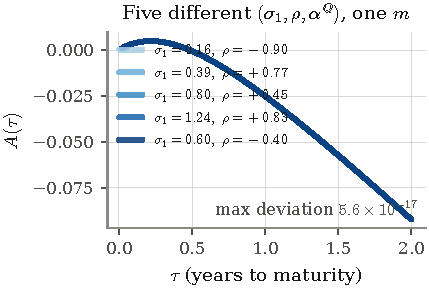
\includegraphics[width=\linewidth]{figures/results/ident2_invariance.pdf}
%         \caption{Five $(\sigma_1,\rho,\longrun^{\mathbb{Q}})$, one $m$}
%         \label{fig:ident_invariance}
%     \end{subfigure}\hfill
%     \begin{subfigure}[b]{0.87\textwidth}
%         \centering
%         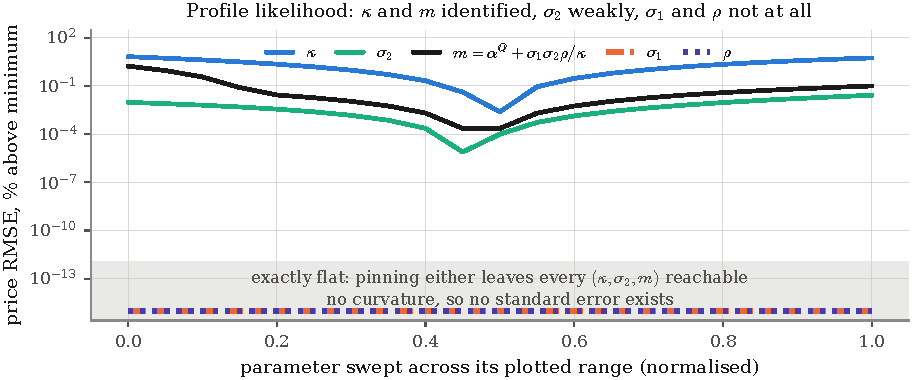
\includegraphics[width=\linewidth]{figures/results/ident1_profile_likelihood.pdf}
%         \caption{Profile likelihood, identified coordinates}
%         \label{fig:ident_profile}
%     \end{subfigure}
%     \caption{The two flat directions of the futures likelihood. (a) $A(\tau)$ evaluated at five different $(\sigma_1, \rho, \longrun^{\mathbb{Q}})$ triples that share a single value of $m = \longrun^{\mathbb{Q}} + \rho\sigma_1\sigma_2/\meanrev$: the curves coincide exactly, so no futures panel can separate them. (b) Profile likelihood over the identified coordinates $(\meanrev, \sigma_2, m)$, each parameter swept across its plotted range and reported as price RMSE above the minimum. Together these are the empirical counterpart of the analytical result in \S\ref{sec:identifiability}.}
%     \Description{Two panels. Left: five overlapping curves of the affine coefficient A against time to maturity, indistinguishable from one another. Right: profile likelihood curves showing clear curvature in kappa, sigma-2 and m.}
%     \label{fig:identifiability}
% \end{figure*}

\subsection{Physics-Enforced Inversion}
\label{sec:pinn_inversion}
The title of this work, \textit{AP-PEN: A Hard-Constrained, Physics-Enforced Network}, highlights a core methodological distinction between informing and enforcing mathematical laws. In a traditional physics-informed approach, a neural network is encouraged to satisfy governing equations through an additional penalty in the loss function~\cite{Raissi2019Physics-informedEquations, Hoshisashi2024Physics-InformedPDEs}. In contrast, a physics-enforced approach builds known mathematical structures directly into the architecture~\cite{rackauckas2020universal}, ensuring constraints are satisfied exactly rather than approximately. Training a neural network to learn the entire pricing function when its components $A(\tau)$ and $B(\tau)$ are deterministic introduces a highly redundant learning problem. 

To resolve this redundancy, we propose the Affine-Partitioned, Physics-Enforced Network (AP-PEN). As detailed in Fig.~\ref{fig:appinn}, AP-PEN translates this physics-enforced paradigm directly into its architecture. The neural layers exclusively parametrise the hidden convenience-yield path $\hat{\delta}_\phi$, while the hardcoded analytical maps $A(\tau)$ and $B(\tau)$ translate this learned path into a futures curve via the exact pricing transform (Eq.~\ref{eq:gs_futures}). Because this construction satisfies the pricing PDE (Eq.~\ref{eq:gs_pde_tau}) by design, it avoids the ``inverse tautology'' problem, where evaluating a PDE with an exact analytical ansatz yields a trivial $0=0$ residual that provides no learning gradient~\cite{rackauckas2020universal}. This structurally eliminates the need for a conventional differential-equation residual penalty~\cite{lu2021deepxde}.

The architecture consists of a single path network, $\hat{\delta}_\phi: t \mapsto \hat{\delta}_\phi(t)$, mapping calendar time directly to the estimated convenience yield. Critically, $\hat{\delta}_\phi$ takes no futures data as input; the inversion is achieved entirely through the training objective rather than the network's forward pass. We detail the architecture below, deferring the composite loss function to \S\ref{sec:multi_obj}.

$\hat{\delta}_\phi$ is a standard feed-forward MLP: three hidden layers of $32$ units each with $\tanh$ activations, and a single linear output unit, taking only normalised calendar time as input. Table~\ref{tab:network_arch} gives the full specification. The \texttt{Dense}/\texttt{MLP} module, the Adam optimiser, and the WamOL gradient-norm loss-balancing scheme (\S\ref{sec:multi_obj}) are all adapted from the WamOL framework of Hoshisashi et al.~\cite{Hoshisashi2024Physics-InformedPDEs, Hoshisashi2024Whack-a-moleSurface}, built to calibrate a Dupire local-volatility surface from three inputs (log-moneyness, time-to-maturity, calendar time) to a non-negative implied volatility. Our adaptation resizes their network to better suit the problem setting: $\hat{\delta}_\phi$ solves a lower-dimensional problem than that in~\cite{Hoshisashi2024Whack-a-moleSurface}, mapping only a single scalar (time) to a single scalar ($\hat{\delta}$); we therefore use a shallower, narrower network, three layers of $32$ units against their four layers of $64$, and drop their output activation entirely, since $\hat{\delta}_\phi$ must be free to take either sign, unlike an implied volatility that Hoshisashi et al.\ constrain to be non-negative with a softplus. The final network consists of $2{,}209$ parameters, which is already vastly overspecified relative to the small number of degrees of freedom in $\delta_t$'s own OU dynamics (Eq.~\ref{sde2}), so no further architecture search was performed.

\begin{table}[tbp]
\centering
\footnotesize
\caption{Path-network architecture and optimisation, contrasted with the WamOL framework (Hoshisashi et al.~\cite{Hoshisashi2024Physics-InformedPDEs, Hoshisashi2024Whack-a-moleSurface}) this work adapts its network code, optimiser, and gradient-balancing scheme from.}
\label{tab:network_arch}
\setlength{\tabcolsep}{3pt}
\begin{tabular}{@{}p{1.65cm}p{2.9cm}p{2.9cm}@{}}
\toprule
 & AP-PEN (this work) & WamOL~\cite{Hoshisashi2024Whack-a-moleSurface} \\
\midrule
Input & Normalised time $t/T$ (1D) & Log-moneyness, $\tau$, calendar time (3D) \\
Hidden layers & 3 & 4 \\
Units per hidden layer & 32 & 64 \\
Hidden activation & $\tanh$ & $\tanh$ \\
Output & $\hat{\delta}_\phi(t)$, linear (signed) & Implied volatility, softplus ($\geq 0$) \\
Weight init & Glorot normal & Glorot normal \\
Optimiser & Adam & Adam + weight decay \\
Learning rate & $9.4\times10^{-3}$, decay $0.82$ every $2{,}657$ steps & $10^{-3}$, decay $0.9$ every $1{,}000$ steps \\
Trainable parameters & 2{,}209 & --- \\
\bottomrule
\end{tabular}
\end{table}

The model takes two primary numerical inputs alongside a set of globally shared parameters. First, the observed data panel: daily records $(S_i, t_i, \{F^{\text{obs}}_{i,k}\}_{k=1}^{N_\tau})$ for $i = 1, \dots, n$ (\S\ref{sec:experimental_design} details both the synthetic and real data formulations). Second, a fixed maturity grid $\{\tau_k\}_{k=1}^{N_\tau}$ that assigns a single time-to-maturity to each contract slot $k$, constant across all observation dates $i$.

We learn the shared parameters $\psi = \{\kappa, \sigma_1, \sigma_2, \rho, \alpha^{\mathbb{P}}\}$ alongside the network weights $\phi$. The risk premium $\lambda_2$ is fixed, while the interest rate $r_i$ enters as observed per-date data for the real panel but remains constant for synthetic experiments (\S\ref{sec:experimental_design}). 

Crucially, we avoid learning the risk-neutral long-run level $\alpha^{\mathbb{Q}}$ directly. Because $\alpha^{\mathbb{P}}$ and $\lambda_2$ interact solely via the measure change $\alpha^{\mathbb{Q}} = \alpha^{\mathbb{P}} - \sigma_2\lambda_2/\kappa$ (Appendix~\ref{app:gs_derivation}), fitting $\alpha^{\mathbb{Q}}$ would create an underdetermined system of infinite $(\alpha^{\mathbb{P}}, \lambda_2)$ pairs. Fixing $\lambda_2$ exogenously breaks this degeneracy, allowing us to derive $\alpha^{\mathbb{Q}}$ exactly from the learned $\alpha^{\mathbb{P}}$ at every step.

To test robustness to misspecified risk premiums, our synthetic experiments generate data with $\lambda_2 = 0.10$ but train using $\lambda_2^{\text{fixed}} = 0.13$ ($+30\%$). For real WTI data, we ensure a fair comparison by fixing $\lambda_2$ to the KF's MLE estimate.

Several parameters require strict physical bounds: positive volatilities, $\sigma_1, \sigma_2 > 0$; valid correlations, $\rho \in [-1, 1]$; and strictly positive mean reversion, $\kappa > 0$. To enforce these realities during unconstrained optimisation, we transform $\sigma_1$ and $\sigma_2$ via a softplus, $\rho$ via $\tanh$, and $\alpha^{\mathbb{P}}$ via the identity. For the mean-reversion rate, we apply a floored softplus: $\kappa = 0.1 + \mathrm{softplus}(\cdot)$.

This $\kappa_{\min} = 0.1$ floor is more than a numerical safeguard. Below $\kappa = 0.1$, the mean-reversion half-life exceeds $6.9$ years~\cite{uhlenbeck1930theory} (Appendix~\ref{app:supplementary}), which is far longer than our maximum $1.88$-year WTI contract (Table~\ref{tab:data_stats}). Because this reversion is too slow to observe in the data, the curve flattens ($B(\tau) \approx -\tau$) and the convenience yield becomes indistinguishable from basic cost-of-carry~\cite{cox1981relation}. The floor simply prevents the optimiser from stalling in this unidentifiable blind spot without restricting realistic market values.

\definecolor{datafill}{RGB}{232,240,250}
\definecolor{datastroke}{RGB}{70,110,160}
\definecolor{netfill}{RGB}{255,255,255}
\definecolor{netstroke}{RGB}{90,90,90}
\definecolor{lossfill}{RGB}{245,238,230}
\definecolor{lossstroke}{RGB}{150,110,70}
\definecolor{sumfill}{RGB}{238,238,238}
\definecolor{anafill}{RGB}{238,234,244}
\definecolor{anastroke}{RGB}{118,98,148}
\definecolor{bpstroke}{RGB}{150,60,55}

\begin{figure*}[tp]
\centering
\resizebox{\textwidth}{!}{%
\begin{tikzpicture}[
    >={Stealth[length=2.2mm]},
    font=\footnotesize,
    flow/.style    ={line width=0.7pt, rounded corners=2.5pt},
    slim/.style    ={line width=0.55pt,rounded corners=2.5pt},
    par/.style     ={line width=0.6pt, draw=anastroke, densely dashed, rounded corners=2.5pt},
    sg/.style      ={line width=0.6pt, draw=netstroke, dash pattern=on 2.4pt off 1.6pt, rounded corners=2.5pt},
    arb/.style     ={line width=0.55pt,draw=lossstroke,densely dashed, rounded corners=2.5pt},
    bp/.style      ={line width=0.75pt,draw=bpstroke,  dashed,          rounded corners=3pt},
    tag/.style     ={font=\scriptsize, inner sep=1.5pt},
    jn/.style      ={circle, fill=black, inner sep=0pt, minimum size=2.4pt},
    dbox/.style    ={draw=datastroke, fill=datafill, rounded corners=2.5pt, line width=0.6pt, align=center, inner sep=3pt},
    abox/.style    ={draw=anastroke,  fill=anafill,  rounded corners=2.5pt, line width=0.6pt, align=center, inner sep=3pt},
    lbox/.style    ={draw=lossstroke, fill=lossfill, rounded corners=2pt,   line width=0.6pt, align=center, inner sep=3pt, text width=36mm},
    cbox/.style    ={lbox, densely dashed},
    sumnode/.style ={draw, fill=sumfill, circle, inner sep=0pt, minimum size=8mm, line width=0.7pt},
]

% ===============================================================
%  LAYOUT CONSTANTS
%  columns: cIn -> cNet -> cTr -> cLoss -> cSum
%  routing channels: xPsi (left), xDel / xFhat (centre), xBP (right)
% ===============================================================
\def\cIn{-0.6}   \def\cNet{3.9}   \def\cTr{7.6}
\def\cLoss{12.4} \def\cSum{15.6}
\def\xPsi{-3.5}  \def\xDel{9.5}   \def\xFhat{9.7}  \def\xBP{17.2}
\def\yBP{7.6}    \def\yTop{6.0}   \def\yNet{3.2}   \def\yMid{1.0}
\def\yAna{-2.0}  \def\yCac{-1.3}  \def\yRcac{-3.2} \def\yPsiBot{-4.5}

% ===============================================================
%  NODES
% ===============================================================
\node[abox,minimum width=36mm,minimum height=20mm] (glob) at (\cIn,\yTop)
     {\textbf{Shared parameters}\\[1pt]
      $\psi=\{\kappa,\sigma_1,\sigma_2,\rho,\alpha^{\mathbb{P}}\}$ \emph{learned}\\[1pt]
      {\scriptsize $\alpha^{\mathbb{Q}}=\alpha^{\mathbb{P}}-\sigma_2\lambda_2/\kappa$ \emph{derived}}\\[-1pt]
      {\scriptsize ($\lambda_2$ fixed)}};

\node[dbox,minimum width=32mm,minimum height=13mm] (data) at (\cIn,\yNet)
     {\textbf{Observed panel}\\[1pt]$(S_i,\,t_i,\,r_i,\,F^{\mathrm{obs}}_{i,k})$};

\node[dbox,minimum width=32mm,minimum height=12mm] (mats) at (\cIn,\yAna)
     {\textbf{Maturity grid}\\[1pt]$\{\tau_k\}_{k=1}^{N_\tau}$};

% --- path network -------------------------------------------------
\node[draw=netstroke,fill=netfill,rounded corners=3pt,line width=0.8pt,
      minimum width=28mm,minimum height=15mm,inner sep=0pt] (pathnet) at (\cNet,\yNet) {};
\begin{scope}[shift={(\cNet,\yNet)}]
  \tikzset{syn/.style={draw=netstroke!50,line width=0.2pt},
           nrn/.style={circle,draw=netstroke,fill=white,minimum size=2.4mm,
                       inner sep=0pt,line width=0.35pt}}
  \coordinate (nin) at (-0.95,0);  \coordinate (nout) at (0.95,0);
  \foreach \k/\yy in {m/-0.34, z/0, p/0.34}{
      \coordinate (a\k) at (-0.32,\yy);  \coordinate (b\k) at (0.32,\yy);}
  \foreach \k in {m,z,p}{\draw[syn] (nin) -- (a\k); \draw[syn] (b\k) -- (nout);}
  \foreach \i in {m,z,p}\foreach \j in {m,z,p}{\draw[syn] (a\i) -- (b\j);}
  \node[nrn] at (nin) {};  \node[nrn] at (nout) {};
  \foreach \k in {m,z,p}{\node[nrn] at (a\k) {}; \node[nrn] at (b\k) {};}
\end{scope}
\node[below=1.2mm of pathnet,align=center] (pathlab)
     {\textbf{Path network} $\hat{\delta}_\phi:\ t\mapsto\hat{\delta}$\\[-2pt]
      {\scriptsize the only trainable network}};

\node[abox,minimum width=34mm,minimum height=15mm] (ABblk) at (\cNet,\yAna)
     {\textbf{Analytic} $A(\tau),\,B(\tau)$\\[1pt]
      {\scriptsize $B(\tau)=-(1-e^{-\kappa\tau})/\kappa$}\\[-1pt]
      {\scriptsize $A(\tau)$: closed form, Eq.~\ref{eq:app_A}}};

\node[abox,minimum width=32mm,minimum height=14mm] (trans) at (\cTr,\yMid)
     {\textbf{Pricing transform}\\[2pt]
      $\hat{F}=S\,e^{\,B(\tau)\hat{\delta}+A(\tau)}$};

% --- loss channels ------------------------------------------------
\node[lbox,minimum height=16mm] (lsde) at (\cLoss,\yTop)
     {$\hat{\mathcal{L}}_{\mathrm{SDE}}$: transition NLL ($\mathbb{P}$, OU)\\[1pt]
      {\scriptsize $-\log p(\hat{\delta}_{i+1}\mid\hat{\delta}_i;\psi)$}\\[-1pt]
      {\scriptsize updates $\alpha^{\mathbb{P}}$ only (Step 2b)}};

\node[cbox,minimum height=14mm] (ldelta) at (\cLoss,\yNet)
     {$\hat{\mathcal{L}}_{h,\delta}$: convenience-yield floor\\[1pt]
      {\scriptsize on $\hat{\delta}_\phi(t_i)$ directly}};

\node[lbox,minimum height=14mm] (ldata) at (\cLoss,\yMid)
     {$\hat{\mathcal{L}}_{\mathrm{data}}$: data misfit\\[1pt]
      {\scriptsize $\|\ln\hat{F}_{i,k}-\ln F^{\mathrm{obs}}_{i,k}\|^2$}};

\node[cbox,minimum height=13mm] (lcac) at (\cLoss,\yCac)
     {$\hat{\mathcal{L}}_{h,\mathrm{cac}}$: cash-and-carry hinge\\[1pt]
      {\scriptsize $\hat{F}_{i,k}$ vs.\ $S_ie^{(r_i+u)\tau_k}$}};

\node[cbox,minimum height=13mm] (lrcac) at (\cLoss,\yRcac)
     {$\hat{\mathcal{L}}_{h,\mathrm{rcac}}$: reverse cash-and-carry hinge\\[1pt]
      {\scriptsize $\hat{F}_{i,k}$ vs.\ $S_ie^{(r_i-\delta_{\max})\tau_k}$}};

\node[sumnode] (sum) at (\cSum,\yMid) {$\Sigma$};

\node[abox,minimum width=28mm,minimum height=16mm] (wamol) at (\cSum,-5.3)
     {\textbf{WamOL}\\[1pt]{\scriptsize channel-level}\\[-1pt]
      {\scriptsize loss balancing}\\[-1pt]
      {\scriptsize (Step 1, every 100 epochs)}\\[-1pt]
      {\scriptsize \emph{inert unless ARB active}}};

% ===============================================================
%  FORWARD EDGES
% ===============================================================
% inputs
\draw[->,flow] (data.east) -- node[tag,above]{$t_i$} (pathnet.west);
\draw[->,flow] (data.south) |- node[tag,above,pos=0.78]{$S_i,\,r_i$} (trans.west);
\draw[->,slim] (mats.east) -- node[tag,above,pos=0.4]{$\tau_k$} (ABblk.west);

% psi bus: glob -> SDE loss, with a hop over the backprop drop.
% The second tag matters: e_SDE READS kappa and sigma_2 but cannot WRITE them
% (both stop-gradiented inside the channel), so only alpha^P is trained here.
\draw[->,par,sharp corners]
      (glob.east) -- node[tag,above,pos=0.08]{$\psi$} (4.42,\yTop)
      arc (180:0:0.18)
      -- node[tag,above,pos=0.62]{\scriptsize $\kappa,\sigma_2$ stop-grad} (lsde.west);
% psi -> analytic block, down the left-hand channel
\draw[->,par] (glob.west) -- (\xPsi,\yTop) -- node[tag,right,pos=0.38]{$\psi$}
      (\xPsi,\yPsiBot) -- (\cNet,\yPsiBot) -- (ABblk.south);

% delta-hat bus
\draw[flow] (pathnet.east) -- node[tag,above,pos=0.10]{$\hat{\delta}$} (\xDel,\yNet);
\node[jn] at (\cTr,\yNet) {};  \node[jn] at (\xDel,\yNet) {};
\draw[->,flow] (\cTr,\yNet) -- (trans.north);
\draw[->,arb]  (\xDel,\yNet) -- (ldelta.west);
\draw[->,sg]   (\xDel,\yNet) -- (\xDel,4.4)
               -- node[tag,above]{$\hat{\delta}$ (stop-grad)} (\cLoss,4.4) -- (lsde.south);

% analytic -> pricing transform
\draw[->,flow] (ABblk.east) -| node[tag,above,pos=0.28]{$A,B$} (trans.south);

% F-hat bus
\draw[->,flow] (trans.east) -- node[tag,above]{$\hat{F}_{i,k}$} (ldata.west);
\node[jn] at (\xFhat,\yMid) {};  \node[jn] at (\xFhat,\yCac) {};
\draw[arb]     (\xFhat,\yMid) -- (\xFhat,\yRcac);
\draw[->,arb]  (\xFhat,\yCac)  -- (lcac.west);
\draw[->,arb]  (\xFhat,\yRcac) -- (lrcac.west);

% ===============================================================
%  LOSS AGGREGATION
% ===============================================================
\draw[->,slim] (lsde.east)   -| node[tag,above,pos=0.20]{$\lambda_{\mathrm{SDE}}$}  (sum.75);
\draw[->,arb]  (ldelta.east) -| (sum.135);
\draw[->,slim] (ldata.east)  -- node[tag,above]{$\lambda_{\mathrm{data}}$} (sum.west);
\draw[->,arb]  (lcac.east)   -| (sum.225);
\draw[->,arb]  (lrcac.east)  -| (sum.265);
\draw[->,par]  ([xshift=10mm]wamol.north) |- node[tag,right,pos=0.18]{$\lambda_\beta$} (sum.320);
\draw[->,flow] (sum.east) -- node[tag,above]{$\hat{\mathcal{L}}$} (\xBP,\yMid);
\node[jn] at (\xBP,\yMid) {};

% ===============================================================
%  BACKPROPAGATION PATH
% ===============================================================
\draw[->,bp] (\xBP,\yMid) -- (\xBP,\yBP)
     -- node[above,font=\scriptsize,text=bpstroke,pos=0.62]
        {backprop:\ $\phi$ (Step 1)\ $\mid$\ $\{\kappa,\sigma_1,\sigma_2,\rho\}$ (Step 2a)\ $\mid$\ $\alpha^{\mathbb{P}}$ (Step 2b)}
     (\cIn,\yBP) -- (glob.north);
\draw[->,bp] (4.6,\yBP) -- (4.6,3.95);

% ===============================================================
%  LEGEND
% ===============================================================
\begin{scope}[shift={(\xPsi,-5.3)},font=\scriptsize,
              key/.style={rounded corners=1.5pt,line width=0.7pt,
                          minimum width=5mm,minimum height=3mm,inner sep=0pt}]
  \node[key,draw=netstroke,  fill=netfill]  (k1) at (0,0)   {};
  \node[anchor=west,inner sep=1.5pt] at (k1.east) {learned network};
  
  \node[key,draw=anastroke,  fill=anafill]  (k2) at (3.0,0) {}; 
  \node[anchor=west,inner sep=1.5pt] at (k2.east) {imposed structure / parameters};
  
  \node[key,draw=datastroke, fill=datafill] (k3) at (7.8,0) {}; 
  \node[anchor=west,inner sep=1.5pt] at (k3.east) {input data};
  
  \node[key,draw=lossstroke, fill=lossfill] (k4) at (10.0,0) {}; 
  \node[anchor=west,inner sep=1.5pt] at (k4.east) {loss channel};
  
  \node[key,draw=lossstroke, fill=lossfill,densely dashed] (k5) at (12.5,0) {}; 
  \node[anchor=west,inner sep=1.5pt] at (k5.east) {AP-PEN (ARB) only};
\end{scope}

\end{tikzpicture}%
}
\caption{The AP-PEN architecture. The observed panel $(S_i, t_i, r_i, F^{\mathrm{obs}}_{i,k})$ and fixed maturity grid $\{\tau_k\}_{k=1}^{N_\tau}$ feed the path network $\hat{\delta}_\phi$ and analytic block, respectively. Shared parameters $\psi = \{\kappa, \sigma_1, \sigma_2, \rho, \alpha^{\mathbb{P}}\}$ (with derived $\alpha^{\mathbb{Q}}$) broadcast to both. The sole learned network, $\hat{\delta}_\phi$, maps calendar time to the estimated convenience yield $\hat{\delta}$, which combines with the analytic maps $A(\tau)$ and $B(\tau)$ to produce the model price $\hat{F}_{i,k}$. Five loss channels exist: data-misfit and SDE transition-NLL (solid boxes, always active), alongside three optional hinge losses (dashed boxes, AP-PEN (ARB) only) enforcing arbitrage bounds and a convenience-yield floor directly on $\hat{\delta}_\phi$. Active channels are summed into $\hat{\mathcal{L}}$ via WamOL gradient balancing (\S\ref{sec:multi_obj}). This balancer is inert for unconstrained variants because the $\hat{\mathcal{L}}_{\mathrm{SDE}}$ gradient into $\phi$ is severed. Backpropagation updates disjoint groups in three alternating steps (\S\ref{sec:alternating}): $\phi$ (full weighted loss), $\{\kappa, \sigma_1, \sigma_2, \rho\}$ (data-misfit only), and $\alpha^{\mathbb{P}}$ (transition-NLL only). Legend: solid arrows carry tensors, dashed purple broadcast parameters, and dashed red trace gradient routes.}
\Description{Block diagram of the AP-PEN architecture: the observed futures panel and maturity grid feed a path network and an analytic block, whose outputs combine in a fixed pricing transform before splitting into five loss channels.}
    \label{fig:appinn}
\end{figure*}

No-arbitrage and economic bounds are introduced as additional loss terms in \S\ref{sec:constraints}, separate from the base composite objective and as a direct extension of the derivative-constrained loss terms developed in~\cite{Hoshisashi2024Physics-InformedPDEs}.

The path network's output is combined with the analytic $A(\tau)$ and
$B(\tau)$ through a pricing transform that is fixed, not learned:
\begin{equation}
    \label{eq:pricing_transform}
    \begin{gathered}
      \hat{F}(S, \hat{\delta}, \tau) = S \exp\!\big(B(\tau)\,\hat{\delta} + A(\tau)\big), \\
      B(\tau) = -\frac{1-e^{-\kappa\tau}}{\kappa}.
    \end{gathered}
\end{equation}

Fixing the shared parameters $\psi$ fully determines the functions $A(\tau)$ and $B(\tau)$, as each uniquely solves an initial value problem in $\tau$ (Eqs.~\ref{eq:gs_ode_B} and \ref{eq:gs_ode_A}). By contrast, the latent state $\delta_t$ is the realised path of a stochastic process (Eq.~\ref{eq:gs_cy}). It cannot be computed analytically from $\psi$ and $t$ alone, as it depends entirely on an unobserved realisation of the driving Brownian motion $W_2^{\mathbb{P}}$~\cite{Schwartz1997TheHedging, duffie2000transform}.

The log-futures relation is linear in $\delta$,
$\ln\hat{F} - \ln S - A(\tau) = B(\tau)\,\delta$ (Eq.~\ref{eq:gs_futures}),
and is therefore directly invertible via least squares at each observation
date. This per-date approach, however, treats every date as an independent
inverse problem and uses no information from neighbouring dates, discarding by
construction the continuous, mean-reverting structure that $\delta$ is known to
obey (Eq.~\ref{sde2}); it also cannot produce a value between observation
dates. A network trained on $t \mapsto \hat\delta_\phi(t)$ across the full
sample is, by contrast, structurally capable of pooling information across
dates through its own inductive bias~\cite{rahaman2019spectral}, and can additionally absorb the DC-PINN
hinge losses (\S\ref{sec:constraints}) directly on the recovered path~\cite{Hoshisashi2024Physics-InformedPDEs},
which the KF's linear-Gaussian structure~\cite{krul2008calibration} (\S\ref{sec:kalman})
cannot accommodate without losing tractability. Whether this pooling capacity
yields a materially better estimate of $\delta_t$ than the per-date baseline
(formalised as an evaluated benchmark in \S\ref{sec:ls_baseline})
is an empirical question addressed in \S\ref{sec:synthetic}.

\subsection{Composite Objective and Loss Balancing}
\label{sec:multi_obj}

The composite loss function $\hat{\mathcal{L}}$ combines two channels adapted to our single-network architecture: a data-fit loss and a path transition negative log-likelihood (NLL) loss. (No PDE-residual or boundary-condition losses are needed, as established in \S\ref{sec:pinn_inversion}.) The optional no-arbitrage hinge penalties are introduced separately in \S\ref{sec:constraints}.

\begin{equation}
\hat{\mathcal{L}} :=
\lambda_{\text{data}} \hat{\mathcal{L}}_{\text{data}}
+ \lambda_{\text{SDE}} \hat{\mathcal{L}}_{\text{SDE}}.
\label{eq:composite}
\end{equation}

The non-negative weights $\lambda_{\text{data}}$ and $\lambda_{\text{SDE}}$ are dynamically adjusted using a WamOL channel-level gradient-norm balancing rule~\cite{Hoshisashi2024Physics-InformedPDEs}. This ensures both channels produce gradient updates of comparable magnitude, preventing one from dominating training. This update mechanism is discussed further in \S\ref{sec:loss_bal}.

The data-fit loss $\hat{\mathcal{L}}_{\text{data}}$ evaluates the mean squared error of the log-price residual across all $N_t$ observation dates $i$ and $N_\tau$ observed maturities $k$. The model price $\hat{F}_{i,k}$ is computed from the spot $S_i$, the estimated convenience yield $\hat{\delta}_\phi(t_i)$, and the time-to-maturity $\tau_k$. Taking the log-futures price ensures $\hat{F}_{i,k}$ enters the pricing transform linearly ($\ln\hat{F}$ is an affine function of $\hat{\delta}$ via $B(\tau)$), yielding a loss surface that is quadratic in $\hat{\delta}$:

\begin{equation}
\begin{gathered}
    \hat{\mathcal{L}}_{\text{data}} = \frac{1}{N_t N_\tau} \sum_{i=1}^{N_t} \sum_{k=1}^{N_\tau} \left\lVert \ln \hat{F}_{i,k} - \ln F^{\text{obs}}_{i,k} \right\rVert^2, \\
    \text{where} \quad \hat{F}_{i,k} := S_i \exp\!\big( B(\tau_k)\,\hat{\delta}_\phi(t_i) + A(\tau_k) \big).
\end{gathered}
    \label{eq:data-loss}
\end{equation}

The SDE channel uses the Ornstein--Uhlenbeck (OU) process (Eq.~\ref{sde2}) to constrain the estimated path $\delta_t$ to its mean-reverting dynamics under $\mathbb{P}$. Because Eq.~\ref{sde2} is linear, it admits a closed-form transition density over each time step $\Delta t$ between consecutive observation dates (derived in Appendix~\ref{app:gs_derivation})~\cite{Schwartz1997TheHedging, vasicek1977equilibrium}:

\begin{equation}
\begin{gathered}
  \delta_{t+\Delta t} \mid \delta_t \sim \mathcal{N}\!\big(m(\delta_t, \Delta t),\, v(\Delta t)\big), \\
  m(\delta_t, \Delta t) = \alpha^{\mathbb{P}} + \big(\delta_t - \alpha^{\mathbb{P}}\big)\,e^{-\kappa \Delta t}, \\
  v(\Delta t) = \frac{\sigma_2^2}{2\kappa} \Big(1 - e^{-2\kappa \Delta t}\Big).
\end{gathered}
\end{equation}

Here, $\mathcal{N}(m, v)$ denotes the normal distribution of the OU transition law~\cite{uhlenbeck1930theory, vasicek1977equilibrium} with mean $m$ and variance $v$. Writing $m_i \coloneqq m(\hat{\delta}_i, \Delta t_i)$ and $v_i \coloneqq v(\Delta t_i)$, the total negative log-likelihood averaged across all $N_p = N_t - 1$ steps is:

\begin{equation}
    \hat{\mathcal{L}}_{\text{SDE}} = \frac{1}{N_p}
  \sum_{i=1}^{N_p} \left(
    \frac{1}{2}\log\!\big(2\pi\, v_i\big)
      + \frac{\big(\hat{\delta}_{i+1} - m_i\big)^2}{2\,v_i} \right).
\end{equation}

Crucially, these two channels route gradients to disjoint subsets of parameters via separate optimiser states. The data-misfit channel exclusively updates the network weights $\phi$ alongside $\{\kappa, \sigma_1, \sigma_2, \rho\}$. The SDE channel exclusively updates $\alpha^{\mathbb{P}}$.

To maintain this strict separation, we apply stop-gradients to $\kappa$, $\sigma_2$, and the predicted path $\hat\delta_\phi$ within the SDE channel~\cite{bradbury2018jax}. This prevents the optimiser from taking mathematical shortcuts. If the SDE loss could alter $\kappa$ and $\sigma_2$, it would drive $\kappa$ toward zero to artificially shrink the transition variance, destroying the parameter fit already established by the price data. Similarly, blocking the gradient to $\hat\delta_\phi$ ensures this channel only calibrates the physical long-run mean $\alpha^{\mathbb{P}}$, rather than interfering with the neural network weights $\phi$ that generate the path itself.

\subsubsection{Parameter Segregation}
\label{sec:alternating}

Rather than updating the path network and all five learned physics
parameters at each epoch, training is split into three sequential steps:
\begin{itemize}
    \item \textbf{Step 1:} Freeze $(\kappa, \sigma_1, \sigma_2, \rho,
    \alpha^{\mathbb{P}})$ and update the path network $\hat{\delta}_{\phi}$
    against the full weighted loss.
    \item \textbf{Step 2(a):} Update $(\kappa, \sigma_1, \sigma_2, \rho)$
    using only the pricing loss $\hat{\mathcal{L}}_{\text{data}}$;
    $\hat{\delta}_{\phi}$ is frozen. Although $\kappa$ and $\sigma_2$ also
    enter the $\mathbb{P}$ transition density in Step 2(b), they are
    measure-invariant and receive their only gradient update here, not there.
    \item \textbf{Step 2(b):} Update the sole $\mathbb{P}$-specific parameter
    $\alpha^{\mathbb{P}}$ using only the path loss
    $\hat{\mathcal{L}}_{\text{SDE}}$; everything else, including $\kappa$ and
    $\sigma_2$, is frozen via stop-gradient.
\end{itemize}
This segregation enforces measure discipline rather than strict identification. It prevents the real-world $\mathbb{P}$ and risk-neutral $\mathbb{Q}$ parameter groups from pulling in conflicting directions during a single update. However, it does not perfectly align parameters with their identifying information. While Step 2(b) correctly isolates $\alpha^{\mathbb{P}}$ using only the transition density, Step 2(a) updates $\sigma_1$ and $\rho$ alongside the identifiable parameters $\kappa, \sigma_2, m$, even though $\sigma_1$ and $\rho$ remain structurally unidentified from cross-sectional data (\S\ref{sec:identifiability}).

We use a separate Adam optimiser for each step instead of zeroing out gradients in a single shared optimiser. Adam builds momentum using a running average of past gradients~\cite{kingma2014adam}. If we feed it a zero gradient for a frozen parameter, Adam interprets this as a signal to slow down, which degrades its momentum. Separate optimisers allow us to completely pause the update process for inactive parameters, keeping their momentum perfectly intact for their next turn.

\subsubsection{Self-Adaptive Loss Balancing}
\label{sec:loss_bal}

The balancing of the composite loss $\hat{\mathcal{L}}$ follows the WamOL algorithm~\cite{Hoshisashi2024Whack-a-moleSurface}. This applies only during Step 1 of the alternating optimisation (\S\ref{sec:alternating}); Steps 2(a) and 2(b) train against single loss channels and require no balancing. Every $100$ epochs, we measure the relative strength of each channel $k \in \{\text{data}, \text{SDE}\}$ using its mean absolute gradient with respect to its parameter support $\Theta_k$ (\S\ref{sec:multi_obj}):

\begin{equation}
g_k(p) := \overline{\big\lvert \nabla_{\Theta_k} \hat{\mathcal{L}}_k(p) \big\rvert}.
\label{eq:gradnorm}
\end{equation}

We use the absolute mean rather than the squared norm of Hoshisashi et al.~\cite{Hoshisashi2024Physics-InformedPDEs} to prevent outlier gradients from dominating during later training stages. The channel weights are then updated via:

\begin{equation}
\begin{gathered}
\lambda_k(p+1) = m\,\lambda_k(p) + (1-m)\, w_k(p), \\
w_k(p) =
\begin{cases}
1, & \text{if } g_k(p) = 0, \\[4pt]
\dfrac{\sum_{j} g_j(p)}{g_k(p)}, & \text{otherwise},
\end{cases}
\end{gathered}
\label{eq:lambda-update}
\end{equation}

where $m \in [0,1)$ is the momentum, $m=0.5$ here, and $j$ indexes all active channels (which expands to $\{\text{data}, \text{SDE}, h\text{-cac}, h\text{-rcac}, h\text{-}\delta\}$ for the AP-PEN (ARB) variant in \S\ref{sec:constraints}). 

Equation~\ref{eq:lambda-update} generalises the scheme in~\cite{Hoshisashi2024Physics-InformedPDEs} by introducing tunable momentum. This applies an exponential moving average (EMA) to smooth the channel weights, cleanly defining the balance between old and new weights (e.g., $m=0.5$ retains $50\%$ of the previous weight). Additionally, if a gradient momentarily vanishes, $g_k(p)=0$, the momentum smoothly nudges $\lambda_k$ toward 1 rather than hard-resetting it.

Because the stop-gradient severs $\hat{\mathcal{L}}_{\text{SDE}}$'s gradient into $\phi$ (\S\ref{sec:multi_obj}), this channel contributes nothing to Step 1. During Step 1, $\psi$ is frozen, meaning the target parameter support $\Theta_{\text{SDE}}$ reduces strictly to $\phi$. Consequently, $g_{\text{SDE}}$ is exactly zero and drops out of the balancing weights.

For the standard AP-PEN variant, this leaves $\hat{\mathcal{L}}_{\text{data}}$ as the single active channel in Step 1. The balancer may therefore have no material effect on path recovery, a consequence we test empirically in \S\ref{sec:synthetic}. However, this limitation vanishes in the AP-PEN (ARB) variant: the no-arbitrage hinge terms $\hat{\mathcal{L}}_{h,\text{cac}}$, $\hat{\mathcal{L}}_{h,\text{rcac}}$, $\hat{\mathcal{L}}_{h,\delta}$ introduced in \S\ref{sec:constraints} maintain live gradients into $\phi$, allowing the balancer to actively manage multiple channels.

\subsection{No-Arbitrage and Economic Constraints}
\label{sec:constraints}
While $\hat{\mathcal{L}}_{\text{data}}$ and $\hat{\mathcal{L}}_{\text{SDE}}$ constrain the network to GS dynamics, neither guarantees the inferred convenience yield $\hat{\delta}_{\phi}$ remains economically rational. To prevent paths that fit the pricing dynamics but violate investor constraints, we introduce an additional loss term, $\hat{\mathcal{L}}_{h}$, generalising the derivative constraints of~\cite{Hoshisashi2024Physics-InformedPDEs} into commodity-specific economic and no-arbitrage inequalities.

These model-free inequalities act independently of the GS dynamics. Following~\cite{zhang2025exact}, we enforce them using a one-sided hinge penalty for constraint violations:
\begin{equation}
\hat{\mathcal{L}}_h = \frac{1}{N} \sum_{i=1}^{N}
\big[ \max\!\big(0, -g(x_i)\big) \big]^2.
\label{eq:hinge}
\end{equation}

The cash-and-carry bounds prevent risk-free profits. Cash-and-carry arbitrage occurs when futures are overpriced relative to spot, allowing a trader to borrow at the risk-free rate, buy the physical asset, and short the future. Reverse cash-and-carry exploits the opposite scenario. Both are evaluated on the same $N_t \times N_\tau$ grid as $\hat{\mathcal{L}}_{\text{data}}$, reusing $\hat{F}_{i,k}$ from Eq.~\ref{eq:data-loss}.

The interest rate $r$, annualised storage cost $u = 0.30$, and convenience yield ceiling $\delta_{\max} = 0.75$ are fixed constants acting as deliberately loose outer guardrails. $\delta_{\max} = 0.75$ accommodates extreme short-term yields during market turmoil, which Gibson and Schwartz observed approaching $100\%$~\cite{Gibson1990StochasticClaims}. Similarly, $u = 0.30$ safely exceeds baseline storage costs, which average $6$--$9\%$ annualised~\cite{stancu2021dynamics, Fama1987CommodityStorage, byun2017speculation}. It also comfortably exceeds the extreme physical storage spikes seen during the April 2020 oil crash, which reached an implied $13$--$22\%$ annualised.\footnote{During the April 2020 crisis, Cushing physical storage lease rates spiked to roughly $\$0.50$--$\$0.55$ per barrel per month \cite{CME2020, Reuters2020}. Annualising this ($\$6.00$--$\$6.60$/year) against contemporaneous March/May 2020 spot prices of approximately $\$27$--$\$46$/bbl yields an implied storage cost of roughly $13$--$22\%$ of spot.}

While these constants align with the literature, we acknowledge a mild use of evaluation data: we cross-checked their specific values against violation rates on our WTI panel. We initially tested dynamically widening the bounds during crisis years (2015, 2016, and 2020) when a tighter $u=0.10$ is frequently violated. However, an ablation study showed this regime-switching offered no measurable improvement in path recovery once training converged, so we adopted universally safe, fixed constants.

With $r$, $u$, and $\delta_{\max}$ held constant, $\kappa$ is the sole learned parameter influencing these bounds via $\hat{F}_{i,k}$. We enforce them through the following two losses:


\begin{equation}
\begin{multlined}
\hat{\mathcal{L}}_{h,\text{cac}} = \frac{1}{N_t N_\tau} \sum_{i=1}^{N_t} \sum_{k=1}^{N_\tau} \\
\Big[ \max\!\Big( 0,\ \hat{F}_{i,k} - S_i\, e^{(r+u)\tau_k} \Big) \Big]^2,
\end{multlined}
\label{eq:cac-loss}
\end{equation}
\begin{equation}
\begin{multlined}
\hat{\mathcal{L}}_{h,\text{rcac}} = \frac{1}{N_t N_\tau} \sum_{i=1}^{N_t} \sum_{k=1}^{N_\tau} \\
\Big[ \max\!\Big( 0,\ S_i\, e^{(r - \delta_{\max})\tau_k} - \hat{F}_{i,k} \Big) \Big]^2.
\end{multlined}
\label{eq:rcac-loss}
\end{equation}

A third hinge acts directly on the latent path to enforce a convenience-yield floor, $\delta_{\min}$. Because the OU process (Eq.~\ref{eq:gs_cy}) has unbounded support, neither $\hat{\mathcal{L}}_{\text{data}}$ nor $\hat{\mathcal{L}}_{\text{SDE}}$ prevents $\hat{\delta}_\phi$ from drifting arbitrarily negative.

While idealised models assume a theoretical floor of $\delta \geq 0$~\cite{Liu2009No-ArbitrageStructures}, enforcing this would artificially bias the model during deep-contango regimes (such as the April 2020 storage-exhaustion crisis, which produced sharply negative yields~\cite{Reuters2020, CME2020}). Instead, we set a loose empirical guardrail of $\delta_{\min} = -0.30$, derived from the lower edge of the simulated paths in \S\ref{sec:experimental_design}.

Like the cash-and-carry bounds, this constraint is enforced via the one-sided squared hinge penalty (Eq.~\ref{eq:hinge}) at every observation date $t_i$. However, it depends solely on the path, without involving spot prices or maturities:
\begin{equation}
\hat{\mathcal{L}}_{h,\delta} = \frac{1}{N_t} \sum_{i=1}^{N_t}
\Big[ \max\!\Big( 0,\ \delta_{\min} - \hat{\delta}_\phi(t_i) \Big) \Big]^2.
\label{eq:delta-floor-loss}
\end{equation}

Hence the full composite loss function for the AP-PEN (ARB) architecture is,

\begin{equation}
\begin{split}
\hat{\mathcal{L}} := {}&
\lambda_{\text{data}} \hat{\mathcal{L}}_{\text{data}}
+ \lambda_{\text{SDE}} \hat{\mathcal{L}}_{\text{SDE}} \\
&+ \lambda_{h,\text{cac}} \hat{\mathcal{L}}_{h,\text{cac}}
+ \lambda_{h,\text{rcac}} \hat{\mathcal{L}}_{h,\text{rcac}} \\
&+ \lambda_{h,\delta} \hat{\mathcal{L}}_{h,\delta}.
\end{split}
\label{eq:composite-full}
\end{equation}

When the no-arbitrage terms are active, $\lambda_{h,\text{cac}}$, $\lambda_{h,\text{rcac}}$ and $\lambda_{h,\delta}$ are balanced by the same gradient-norm mechanism of Eqs.~\ref{eq:gradnorm}--\ref{eq:lambda-update}, with the channel index $k$ there extended to range over $\{\text{data}, \text{SDE}, h\text{-cac}, h\text{-rcac}, h\text{-}\delta\}$ rather than the two-channel set of \S\ref{sec:multi_obj}; they are not fixed weights.

\subsection{Closed-Form Least-Squares Baseline}
\label{sec:ls_baseline}

Because $\ln \hat{F}$ is linear in $\delta_t$ (Eq.~\ref{eq:pricing_transform}), the inversion admits a closed-form solution at each date for any fixed $\psi$. Minimising the log-price residual (Eq.~\ref{eq:data-loss}) over the scalar $\delta_t$ yields the per-date ordinary least-squares (LS) estimate:
\begin{equation}
  \label{eq:ls_delta}
  \hat{\delta}^{\text{LS}}_t
  = \frac{\sum_{k=1}^{N_\tau} B(\tau_k)\big(
      \ln F^{\text{obs}}_{t,k} - \ln S_t - A(\tau_k)\big)}
         {\sum_{k=1}^{N_\tau} B(\tau_k)^2}.
\end{equation}
Profiling out the identifiable parameters $(\kappa, \sigma_2, m)$ (\S\ref{sec:identifiability}) yields the exact maximum-likelihood estimator under i.i.d.\ Gaussian log-price noise (Eq.~\ref{eq:noise-model})~\cite{Schwartz1997TheHedging}.

This benchmark serves as a natural control to test whether the neural parameterisation adds value. It represents exactly what AP-PEN reduces to if the path network provides nothing beyond a per-date fit. By construction, this date-by-date solver sacrifices the core advantages of the network (\S\ref{sec:pinn_inversion}): pooling information across neighbouring dates via inductive bias, interpolating between observations, and applying path-dependent hinge penalties (\S\ref{sec:constraints}).


\subsection{Kalman Filter Baseline}
\label{sec:kalman}

Because the path network $\hat{\delta}_\phi$ trains on the full sample, AP-PEN acts as a \textit{smoother} with access to future information. In contrast, the KF baseline~\cite{Schwartz1997TheHedging} is causal, using information only up to $t_i$. Any performance gap between the methods stems partly from this asymmetry. A true like-for-like comparison requires the non-causal Rauch--Tung--Striebel (RTS) smoother~\cite{rauch1965maximum}, which we leave to future work (\S\ref{sec:future_work}).

Our KF implementation follows Krul~\cite{krul2008calibration}. The state is the joint latent pair $(x_t, \delta_t)$, where $x_t=\ln S_t$. Both are inferred solely from the futures curve, using the true spot price only to initialise $x_0$. The transition equation applies the Euler--Maruyama discretisation~\cite{maruyama1955continuous} from our Monte Carlo generation (\S\ref{sec:experimental_design}), evaluated over true calendar steps. The measurement equation uses the log-form of the pricing transform (Eq.~\ref{eq:pricing_transform}); because this is exactly linear in $(x_t, \delta_t)$, no Extended or Unscented KF is required. 

To handle varying liquidity, we estimate separate noise variances for each maturity slot, and we seed $\delta_0$ using a model-free basis estimate from the two nearest maturities. Enforcing the measure discipline of \S\ref{sec:gs_model}, we share only $\{\kappa,\sigma_1,\sigma_2,\rho\}$ across measures and derive $\alpha^{\mathbb{Q}} = \alpha^{\mathbb{P}}-\sigma_2\lambda_2/\kappa$. The filter is ultimately calibrated on the WTI panel (\S\ref{sec:real_data}) via maximum likelihood over the prediction-error decomposition.


\subsection{Data and Experimental Design}
\label{sec:experimental_design}

\paragraph{Simulated Data.} Real-world futures data lacks a true, observable convenience yield $\delta_t$, making it impossible to directly score state-estimation accuracy. To resolve this, we generate synthetic paths for the spot price $S_t$ and convenience yield by simulating their $\mathbb{P}$-measure SDEs (Eqs.~\ref{sde1}~\&~\ref{sde2}). Applying the Euler--Maruyama discretisation~\cite{maruyama1955continuous, higham2001algorithmic} to $\delta_t$ and the log-spot price $X = \ln S_t$ yields:

\begin{equation}
X_{n+1} = X_n + \left(\mu - \delta_n - \tfrac{1}{2}\sigma_1^2\right)\Delta t + \sigma_1\,\Delta W_{1,n}
\label{eq:x_discrete_em}
\end{equation}
\begin{equation}
    \delta_{n+1} = \delta_n + \kappa\left(\alpha_P - \delta_n\right)\Delta t + \sigma_2\,\Delta W_{2,n}
    \label{eq:delta_discrete_em}
\end{equation}

for $n = 0,\dots,N-1$, with $\Delta W_{1,n},\Delta W_{2,n}\sim\mathcal{N}(0,\Delta t)$ and $\mathrm{Cov}(\Delta W_{1,n},\Delta W_{2,n})=\rho\,\Delta t$. The spot price is then recovered as $S_n = \exp(X_n)$.

Evaluating the closed-form pricing equation (Eq.~\ref{eq:pricing_transform}) at each simulated state $(S_n, \delta_n)$ produces the full futures curve at every date. Fig.~\ref{fig:mc_term_structure_3d} visualises this term structure as a continuous surface, showing the curve tilt between contango and backwardation as $\delta_t$ cycles through its OU dynamics. To mimic real markets, we inject observation noise $\varepsilon$ to create the noisy panel fed to AP-PEN:

\begin{equation}
\begin{gathered}
\ln \hat{F}_{\text{obs}}(\tau) = \ln F(\tau, S, \delta) + \varepsilon, \\
\varepsilon \sim \mathcal{N}(0,\sigma_\varepsilon^2)
\end{gathered}
\label{eq:noise-model}
\end{equation}

Because the closed-form term-structure slope is an exact affine function of $\delta_t$, this noise is the sole source of ambiguity when recovering $\delta_t$ from the panel. Fig.~\ref{fig:mc_identifiability_scatter} overlays the noisy slope on this exact relationship, demonstrating that the inversion problem remains well posed. We simulate $100$ paths over a $10$-year horizon with an initial spot $S_0 = 100$. Physical GS parameters are drawn from~\cite{Schwartz1997TheHedging}, while $r$ and $\lambda_2$ are fixed estimates. Table~\ref{tab:gs-mc-params} details the complete simulation configuration.

\begin{table*}[tp]
\centering
\caption{GS parameters used for Monte Carlo synthetic data generation.}
\label{tab:gs-mc-params}
\begin{threeparttable}
\resizebox{\textwidth}{!}{%
\begin{tabular}{llll@{\hspace{2em}}llll}
\toprule
\multicolumn{4}{c}{\textit{$\mathbb{P}$-measure (physical dynamics)}} & \multicolumn{4}{c}{\textit{$\mathbb{Q}$-measure (pricing) \& simulation}} \\
\cmidrule(r){1-4} \cmidrule(l){5-8}
Symbol & Description & Value & Source & Symbol & Description & Value & Source \\
\midrule
$\mu$      & Total expected return on spot          & $0.142$ & \multirow{6}{*}{Schwartz~\cite{Schwartz1997TheHedging}\tnote{a}} & $r$                        & Risk-free rate                     & $0.05$  & Assumed \\
$\kappa$   & Mean-reversion speed of $\delta_t$     & $1.876$ & & $\lambda_2$                & Market price of conv.\ yield risk  & $0.10$  & Assumed\tnote{b} \\
$\alpha_P$ & Long-run mean of $\delta_t$ under $\mathbb{P}$ & $0.106$ & & $\lambda_2^{\text{fixed}}$ & Risk premium fixed during training & $0.13$  & $+30\%$ misestimate (\S\ref{sec:pinn_inversion}) \\
$\sigma_1$ & Spot volatility                        & $0.393$ & & $\alpha_Q$                 & Long-run mean of $\delta_t$ under $\mathbb{Q}$ & derived & $\alpha_P - \sigma_2\lambda_2/\kappa$ \\
$\sigma_2$ & Convenience yield volatility           & $0.527$ & & $\sigma_\varepsilon$       & Observation noise std.\ (log-price)& $0.01$  & Chosen \\
$\rho$     & Correlation, $dW_1$ and $dW_2$         & $0.766$ & & $S_0$                      & Initial spot price                 & $100$   & Chosen \\
           &                                        &         & & $T$                        & Simulated horizon (years)          & $10$    & Chosen \\
           &                                        &         & & $N$                        & Number of time steps               & $1000$  & Chosen \\
           &                                        &         & & $M$                        & Number of simulated paths          & $100$   & Chosen \\
\bottomrule
\end{tabular}%
}
\begin{tablenotes}
\footnotesize
\item[a] Table VI, column I: WTI F1-F9, 1/2/85-12/17/95~\cite{Schwartz1997TheHedging}.
\item[b] Not pinned by any no-arbitrage condition; $\lambda_2$ is absorbed into $\alpha_Q$ and identified only through calibration.
\end{tablenotes}
\end{threeparttable}
\end{table*}


\begin{figure*}[tp]
%% Authored at 4.83in and 2.79in. Side by side they total 7.62in against a
%% 7.0in text width, so both take a matched 0.90x -- reduced together, never
%% enlarged, so their label sizes stay comparable.
\begin{subfigure}[b]{0.62\textwidth}
    \centering
    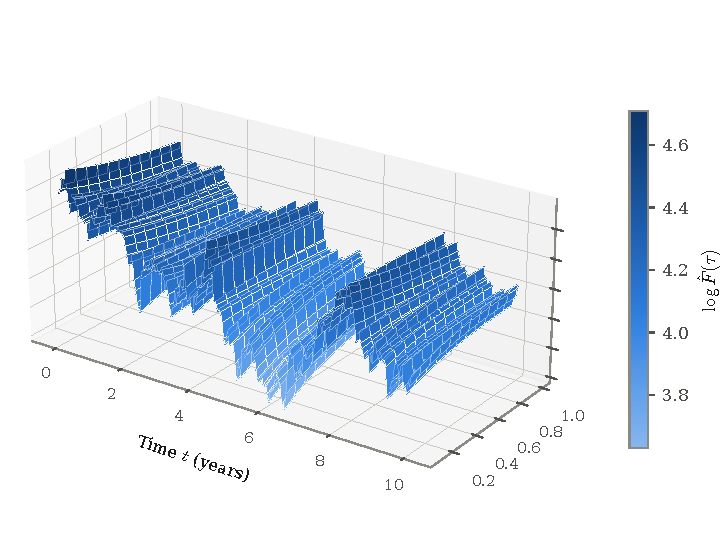
\includegraphics[width=\linewidth]{figures/methodology/mc2c_term_structure_3d.pdf}
    \subcaption{}
    \label{fig:mc_term_structure_3d}
\end{subfigure}\hfill
\begin{subfigure}[b]{0.36\textwidth}
    \centering
    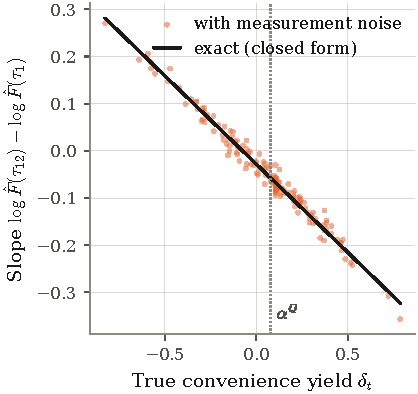
\includegraphics[width=\linewidth]{figures/results/mc3b_identifiability_scatter.pdf}
    \subcaption{}
    \label{fig:mc_identifiability_scatter}
\end{subfigure}
\caption{The simulated term structure as a 3D surface (a), showing the curve tilt through the OU cycle of $\delta_t$; and the term-structure slope as an exact affine function of $\delta$ (closed form, b), with measurement noise overlaid.}
\Description{Two panels: a three-dimensional surface of the simulated futures term structure over maturity and date, and a scatter of term-structure slope against the convenience yield showing an exact linear relationship with noise overlaid.}
    \label{fig:mc_term_structure_and_slope}
\end{figure*}


\paragraph{Evaluation Scheme.} Our evaluation spans two phases: Phase 1 validates against the Monte Carlo ground truth $(\delta_t, S_t)$ (Eqs.~\ref{eq:x_discrete_em}--\ref{sde2}), while Phase 2 tests out-of-sample pricing on a real WTI calendar holdout (\S\ref{sec:real_data}). We compare six models (an MLP, AP-PEN without loss balancing, standard AP-PEN, AP-PEN with no-arbitrage hinge terms, the LS baseline of \S\ref{sec:ls_baseline}, and a KF) across state RMSE, constraint activity rate, price RMSE, benchmark correlation, and convergence diagnostics.

To ensure robustness, all neural network results are reported as the mean $\pm$ standard deviation across five independent random seeds ($42, 7, 123, 2024, 31337$). The LS and KF baselines are deterministic and therefore carry no seed variance.

%% ----------------------------------------------------------------------
%% FIGURE PLACEHOLDER -- synthetic vs. real maturity distributions, and the real term structure
%% Files: figures/data_comparison/data_maturity_distribution_{synthetic,real}.pdf; figures/raw_data/{real_data_term_structure_3d, real_data_basis_surface, real_data_delta_proxy}.pdf
%% Uncomment the block below to include it (select and Ctrl+/ in Overleaf).
%% ----------------------------------------------------------------------
% \begin{figure*}[tp]
%     \centering
%     \begin{subfigure}[b]{0.49\textwidth}
%         \centering
%         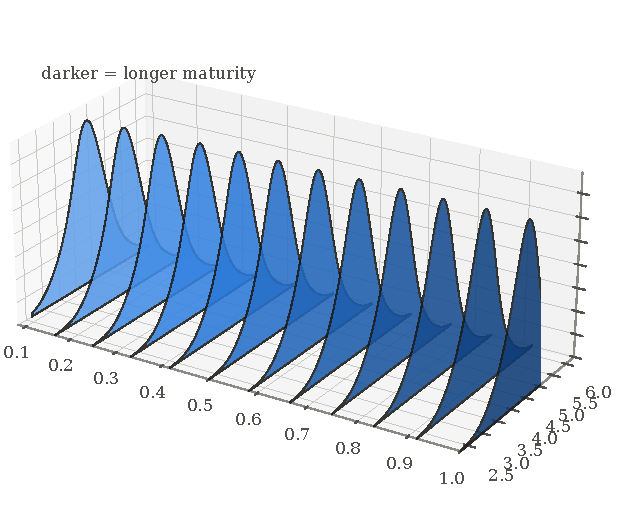
\includegraphics[width=\linewidth]{figures/data_comparison/data_maturity_distribution_synthetic.pdf}
%         \caption{Synthetic panel}
%         \label{fig:maturity_dist_synth}
%     \end{subfigure}\hfill
%     \begin{subfigure}[b]{0.49\textwidth}
%         \centering
%         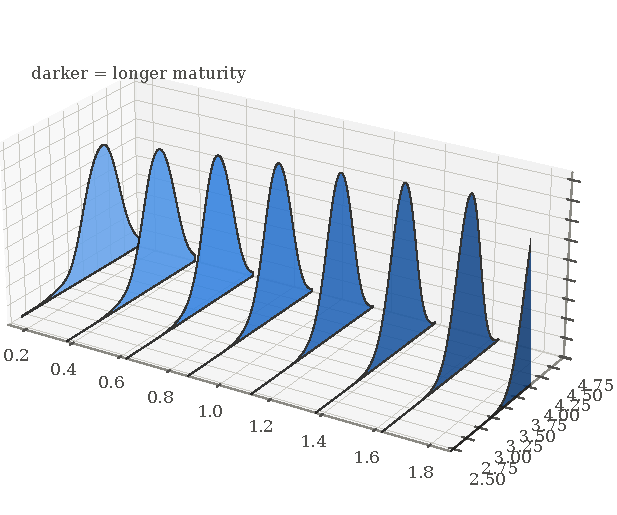
\includegraphics[width=\linewidth]{figures/data_comparison/data_maturity_distribution_real.pdf}
%         \caption{Real WTI panel}
%         \label{fig:maturity_dist_real}
%     \end{subfigure}
%     \caption{Distribution of observed log-futures prices across maturity slots, as a 3D ridgeline: one Gaussian-KDE density per maturity for (a) the synthetic panel and (b) the real WTI panel. Read alongside Fig.~\ref{fig:mc_identifiability_scatter}, these establish how far the simulated panel's coverage of the maturity axis resembles the real one.}
%     \Description{Two three-dimensional ridgeline plots, each stacking one smoothed density curve per maturity slot along a depth axis.}
%     \label{fig:maturity_distribution}
% \end{figure*}
%
\paragraph{Real WTI panel.} We use dated quarterly WTI futures (Mar/Jun/Sep/Dec, Cushing delivery) instead of rolling generics to compute an exact time-to-maturity $\tau = (T-t)/365$.\footnote{Entitlement restrictions blocked chain expansion in Refinitiv Workspace~\cite{refinitiv2026eikon}, requiring individual contract queries. Archive RIC suffixes vary: single-digit year with \texttt{\^{}1} (2015--2019), single-digit year with \texttt{\^{}2} (2020--2023), and two-digit year with \texttt{\^{}2} (2024--2026).} Expiries follow the CME last-trading-day rule, perfectly matching Refinitiv's expiry field across $36$ cross-validated contracts~\cite{refinitiv2026eikon}. Spot prices and financing rates come from the CLc1 continuation and FRED DGS3MO series~\cite{refinitiv2026eikon, fred2026dgs3mo}, respectively. We drop the 2020-04-20 observation because its $-\$37.63$ front-month print is a liquidation artefact, and several model constructs require $S_t > 0$.

For each date, we keep the eight nearest contracts and drop any dates that have fewer than eight. To make the data easier to process in batches, we fix the time-to-maturity $\tau$ for each of the eight slots to its overall average, rather than tracking the exact days remaining as they shrink over time. While this makes training simpler, it does lose some temporal accuracy, which we discuss as a limitation in \S\ref{sec:future_work}.

Table~\ref{tab:data_stats} shows how we filtered the raw data down to the final $2{,}770$ dates (2 January 2015 to 19 February 2026). Fig.~\ref{fig:wti_market_state} plots the spot price and financing rate of this final dataset, and \S\ref{sec:real_data} visualises its term structure.

\begin{table*}[tp]
\centering
\caption{Descriptive statistics for the real WTI futures panel.}
\label{tab:data_stats}
\begin{threeparttable}
\resizebox{\textwidth}{!}{%
\begin{tabular}{lll}
\toprule
Statistic & Raw panel (Refinitiv \& FRED) & Model panel (post-construction)\tnote{a} \\
\midrule
Date range                          & 2015-01-02 -- 2026-06-29         & 2015-01-02 -- 2026-02-19 \\
Trading dates                       & $2{,}891$                        & $2{,}770$ ($95.8\%$ of dates with valid spot/rate)\tnote{b} \\
Unique contract tickers             & $52$                              & --- \\
Live contracts quoted per date      & min $6$, mode $8$, max $9$        & fixed at $8$ (ranked by $\tau$, ascending)\tnote{c} \\
Maturity slots $K$                  & ---                                & $8$ \\
Time to maturity $\tau$ (years)     & $[0.003,\ 2.00]$                  & per-slot mean $\tau \in \{0.125, 0.375, 0.625, 0.875, 1.125, 1.376, 1.626, 1.876\}$ \\
Settlement price (\$/bbl)           & $[11.57,\ 117.15]$                & $[11.57,\ 117.15]$ \\
Spot price (\$/bbl)                 & $[10.01,\ 123.70]$                & $[10.01,\ 123.70]$ \\
Risk-free rate $r$                  & $[0.000,\ 0.0563]$, mean $0.0208$ & $[0.000,\ 0.0563]$, mean $0.0208$ \\
\bottomrule
\end{tabular}%
}
\begin{tablenotes}
\footnotesize
\item[a] The model panel is the rectangular array (dates $\times$ 8 maturities) generated by \texttt{get\_data\_wti} for training (\S\ref{sec:real_data}).
\item[b] We drop $121$ of the $2{,}891$ raw dates. One is 2020-04-20 (missing spot/rate data). The other $120$ have fewer than $8$ live contracts. Most of these ($90$) occur at the end of the sample, which is why the model panel ends early on 19 February 2026. The remaining $30$ are scattered mostly between 2015 and 2019.
\item[c] If a date has more than $8$ quoted contracts, we retain the $8$ nearest maturities. Dates with fewer than $8$ are dropped (see note b).
\end{tablenotes}
\end{threeparttable}
\end{table*}


\begin{figure*}[tp]
    \centering
    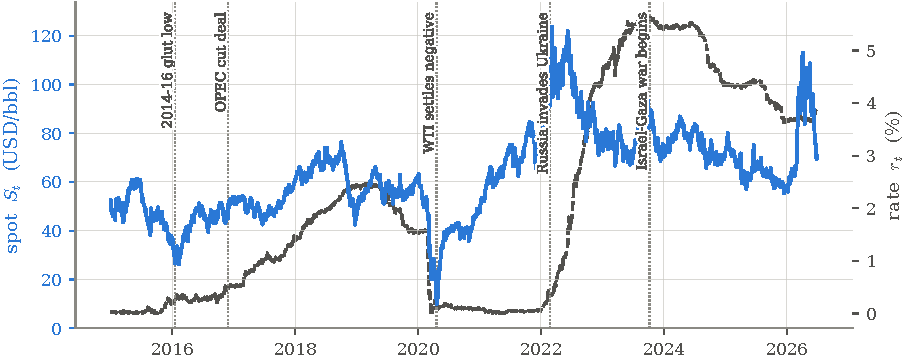
\includegraphics[width=0.87\textwidth]{figures/methodology/real_data_market_state.pdf}
    \caption{WTI spot price $S_t$ and risk-free rate $r_t$ over the sample, 2 January 2015 -- 29 June 2026, with major oil-market events marked for context (2014--16 glut low, 2016 OPEC cut deal, the April 2020 negative-WTI print, Russia's invasion of Ukraine, and the start of the Israel--Gaza war).}
    \Description{Time series of the WTI spot price and the risk-free rate from 2015 to 2026, annotated with major oil-market events.}
    \label{fig:wti_market_state}
\end{figure*}



%% ════════════════════════════════════════════════════════════════════════════
%% 4. RESULTS AND DISCUSSION
%% ════════════════════════════════════════════════════════════════════════════

\section{Results and Discussion}
\label{sec:results}
The evaluation proceeds in two phases: Phase 1 trains on Monte Carlo-simulated data with known GS parameters (Table~\ref{tab:gs-mc-params}), allowing exact error measurement across four model variants (an MLP, AP-PEN without loss balancing, vanilla AP-PEN, and AP-PEN with no-arbitrage constraints), while Phase 2 trains on real WTI futures data, evaluating performance against a KF baseline since true latent states are unobservable. At each phase the model variants are contrasted with the LS approach detailed in \S\ref{sec:ls_baseline}, and throughout this section we evaluate both the recovered latent state path $\hat{\delta}$ and the structural parameters $\psi$, as well as the efficacy of the cash-and-carry, reverse cash-and-carry, and convenience yield floor constraints, noting that a model's accuracy in one does not guarantee success in the other.

\subsection{Synthetic Validation}
\label{sec:synthetic}
Fig.~\ref{fig:path_repeat_recovery_noise_comparison} demonstrates AP-PEN's highly accurate recovery of the latent convenience yield $\delta_t$. This state inversion remains remarkably robust to market noise: a tenfold increase ($\sigma_{\text{noise}} = 0.10$) causes only a modest correlation drop from $0.982$ to $0.972$.

\begin{figure}[tbp]
    \centering
    %% Authored at 2.84in; 0.85\columnwidth = 2.83in, so both render at 1.00x
    %% with their native aspect ratio. Stacked because two of them side by side
    %% in one column would be ~1.6in each.
    \begin{subfigure}[t]{\columnwidth}
        \centering
        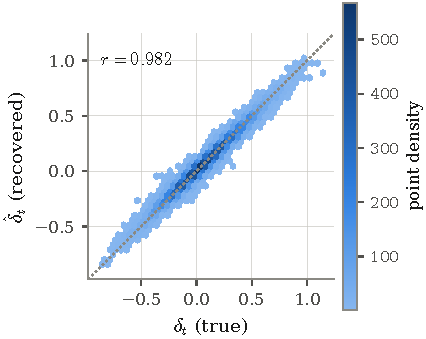
\includegraphics[width=0.85\columnwidth]{figures/results/pinn3c_path_repeat_recovery.pdf}
        \subcaption{$\sigma_{\text{noise}} = 0.01$}
        \label{fig:path_repeat_recovery_noise001}
    \end{subfigure}

    \vspace{0.25cm}

    \begin{subfigure}[t]{\columnwidth}
        \centering
        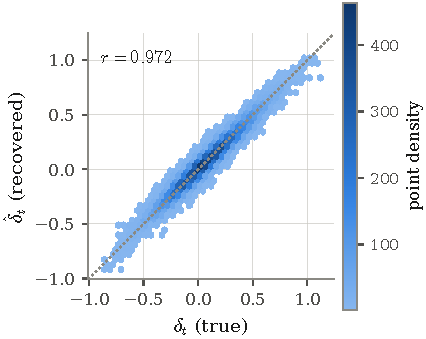
\includegraphics[width=0.85\columnwidth]{figures/results/pinn3c_path_repeat_recovery_noise0.10.pdf}
        \subcaption{$\sigma_{\text{noise}} = 0.10$}
        \label{fig:path_repeat_recovery_noise010}
    \end{subfigure}

    \caption{True vs.\ recovered $\delta_t$ pooled across $20$ independent paths ($20{,}020$ points each), shown as a hexbin density against the $y=x$ perfect-recovery line. Comparing (a) baseline to (b) $10\times$ observation noise reveals only modest degradation ($r = 0.982 \to 0.972$; RMSE = $0.050 \to 0.063$), demonstrating that AP-PEN's inversion remains robust even with significantly noisier data.}
    \Description{Two hexbin density plots of true against recovered convenience yield, at baseline and at ten times the observation noise, both clustered along the line of perfect recovery.}
    \label{fig:path_repeat_recovery_noise_comparison}
\end{figure}

However, whilst Fig.~\ref{fig:path_repeat_recovery_noise_comparison} shows an accurate $\delta$ recovery across noise increments, Table~\ref{tab:synth_delta_recovery} tells a different story. The closed-form LS beats every neural variant on $\delta$-RMSE ($0.00873$ vs $0.0509$--$0.0655$), by $5.8\times$ against the best neural variant (MLP) and up to $7.5\times$ against AP-PEN (ARB), and reproduces $102.8\%$ of the true path's increment-to-increment standard deviation, against $24$--$32\%$ for the neural variants. Each neural network recovers $\delta_t$'s level correctly but does not replicate its dynamics, over-smoothing the convenience yield path and failing to capture the granular variation that the LS approach reproduces almost exactly. This is consistent with spectral bias: a feature of the optimisation method rather than a lack of training, whereby the model settles for predicting close to the conditional mean rather than the fine variance~\cite{rahaman2019spectral}. On accuracy alone, then, AP-PEN buys nothing over a trivial per-date solve; whether the no-arbitrage constraints justify the network regardless is examined next.

\begin{table}[tbp]
\centering
\footnotesize
\caption{Latent-state recovery on the synthetic futures panel, run across five independent seeds. The closed-form baseline solves Eq.~\ref{eq:ls_delta} with $\psi$ profiled out, requiring no training; MLP and AP-PEN are statistically indistinguishable here. The increment ratio measures the standard deviation of the recovered day-to-day changes relative to the true changes, effectively comparing the volatility of the model's estimates against the actual data.}
\label{tab:synth_delta_recovery}
\footnotesize
\resizebox{\columnwidth}{!}{%
\begin{tabular}{lrrrr}
\toprule
Method & $\delta$-RMSE & Correlation & Increment ratio & Training \\
\midrule
No-skill (constant at the mean) & $0.24552$ & --- & $0\%$ & --- \\
\midrule
MLP           & $0.05093 \pm 0.00367$ & $0.9781 \pm 0.0032$ & $32.1 \pm 2.7\%$ & 40k epochs \\
AP-PEN        & $0.05295 \pm 0.00196$ & $0.9764 \pm 0.0018$ & $31.7 \pm 2.0\%$ & 40k epochs \\
AP-PEN (ARB)  & $0.06552 \pm 0.00330$ & $0.9705 \pm 0.0052$ & $24.2 \pm 2.0\%$ & 40k epochs \\
\midrule
Closed-form LS (exact MLE) & $\mathbf{0.00873}$ & $\mathbf{0.9994}$ & $\mathbf{102.8\%}$ & none \\
\bottomrule
\end{tabular}%
}
\end{table}

While the hidden state recovery succeeds, learning the underlying structural parameters $\psi$ exposes a structural identifiability limit (Appendix~\ref{app:supplementary}, Fig.~\ref{fig:param_recovery_appendix}). The pricing transform (Eq.~\ref{eq:pricing_transform}) bundles $\sigma_1$ and $\rho$ together with $\sigma_2$ through the cross-term $\rho\sigma_1\sigma_2$, and drops the isolated spot volatility entirely, since $\partial^2\hat F/\partial S^2 = 0$. Consequently, these unidentified parameters, $\sigma_1$, $\rho$, $\rho\sigma_1\sigma_2$, $\alpha^{\mathbb{Q}}$, show massive coefficients of variation across draws, from $49\%$ to $265\%$ (Table~\ref{tab:synth_psi_multidraw}): precisely the degeneracy predicted analytically in \S\ref{sec:identifiability}, and not a symptom of insufficient training. In stark contrast, the identified coordinates $\kappa$, $\sigma_2$, and $m$ converge tightly to their true values, with coefficients of variation between $1.3\%$ and $9.0\%$, confirming empirically that a futures panel determines exactly these three quantities and no more.

\begin{table*}[tp]
\centering
\caption{Recovered $\psi$ on the synthetic panel against the true and
initialised values, with the closed-form profiled MLE of \S\ref{sec:ls_baseline}
for reference. All columns are the single path at seed $42$, final epoch of
40k, except AP-PEN, reported as mean $\pm$ std (CV) over 20 independent Monte
Carlo noise draws (path recovery: $\delta$-RMSE $0.0504\pm0.0030$). Rows are
grouped by whether the futures cross-section identifies the quantity
(\S\ref{sec:identifiability}). MLP has no $\hat{\mathcal{L}}_{\text{SDE}}$
channel, so its $\alpha^{\mathbb{P}}$ never leaves its initial value.}
\label{tab:synth_psi_recovery}
\label{tab:synth_psi_multidraw}
\resizebox{\textwidth}{!}{%
\begin{tabular}{lrrrrrrr}
\toprule
Parameter & True & Init & Closed-form LS & MLP & AP-PEN (no bal.) & AP-PEN (20-draw) & AP-PEN (ARB) \\
\midrule
$\kappa$      & $1.8760$ & $2.8140$ & $1.8881$ & $1.8516$ & $1.8743$ & $1.8476 \pm 0.0242\ (1.3\%)$ & $1.5874$ \\
$\sigma_2$    & $0.5270$ & $0.6851$ & $0.5206$ & $0.5087$ & $0.5180$ & $0.5425 \pm 0.0489\ (9.0\%)$ & $0.0582$ \\
$m$           & $0.1625$ & --- & $0.1607$ & $0.1605$ & $0.1606$ & $0.1654 \pm 0.0063\ (3.8\%)$ & $0.1251$ \\
\midrule
$\sigma_1$    & $0.3930$ & $0.2751$ & --- & $0.6519$ & $0.4972$ & $0.5511 \pm 0.2725\ (49.4\%)$ & $0.7406$ \\
$\rho$        & $0.7660$ & $0.4596$ & --- & $0.8387$ & $0.8184$ & $0.7002 \pm 0.3577\ (51.1\%)$ & $0.8509$ \\
$\rho\sigma_1\sigma_2$ & $0.1586$ & $0.0866$ & --- & $0.2781$ & $0.2108$ & $0.2424 \pm 0.1712\ (70.6\%)$ & $0.0367$ \\
$\alpha^{\mathbb{Q}}$ & $0.0779$ & $0.1379$ & --- & $0.0103$ & $0.0482$ & $0.0346 \pm 0.0917\ (265\%)$ & $0.1020$ \\
$\alpha^{\mathbb{P}}$ & $0.1060$ & $0.0460$ & --- & $0.0460$ & $0.0841$ & $0.0728 \pm 0.0919\ (126\%)$ & $0.1068$ \\
\midrule
$e_{\text{cac}}$ (final) & \multicolumn{3}{c}{---} & $3.31\times10^{-4}$ & $2.30\times10^{-4}$ & $2.30\times10^{-4}$ & $0.00$ \\
\bottomrule
\end{tabular}%
}
\end{table*}

Table~\ref{tab:synth_psi_recovery} shows that introducing the no-arbitrage guardrails in the AP-PEN (ARB) variant markedly degrades this otherwise strong parameter recovery ($\sigma_2$ alone moves from $0.518$ to $0.058$, an order of magnitude off). This reflects a property of the guardrail, not a flaw in the synthetic data or a model failure. Because the simulated panel was generated independently of the storage-cost bound $u$ (\S\ref{sec:constraints}), a small fraction of the raw points, while fully consistent with the model's own arbitrage-free pricing, already sit outside this deliberately loose guardrail: the observed synthetic panel breaches the cash-and-carry ceiling on $0.70\%$ of its points, and the \emph{true} $\delta_t$ of the data-generating process falls below $\delta_{\min}$ on $4.30\%$ of dates. The unconstrained variants simply reproduce these points in fitting the data closely. AP-PEN (ARB), however, is explicitly penalised for them: its accuracy drop reflects the cost of actively fighting the true data-generating process to enforce an economic guardrail, rather than a failure of the constraint mechanism. Fig.~\ref{fig:training_losses} (Appendix~\ref{app:supplementary}) shows this directly: the hinge losses converge toward zero over training precisely as the data-misfit and SDE-transition losses do, confirming the degraded $\psi$ recovery is the price of a converged constraint rather than a sign of a divergent run. On synthetic data, then, the constraints are demonstrably costly and, by construction, cannot be shown to pay off: the guardrail is calibrated for real-world storage economics the simulator was not built to respect. Section~\ref{sec:real_data} asks the question this section leaves open.


%% ----------------------------------------------------------------------
%% FIGURE PLACEHOLDER -- single-path recovery, variant ablation, and the 20-draw spread
%% Files: figures/pinn/{pinn2a_delta_recovery, pinn2b_delta_recovery_error, pinn2c_delta_recovery_all_variants, pinn3a_path_repeat_errors, pinn3b_path_repeat_rmse}.pdf
%% Uncomment the block below to include it (select and Ctrl+/ in Overleaf).
%% ----------------------------------------------------------------------
% \begin{figure*}[tp]
%     \centering
%     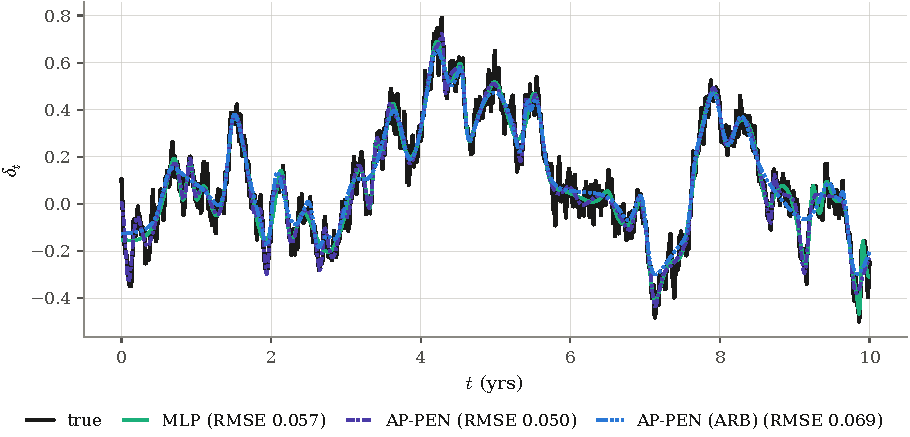
\includegraphics[width=0.87\textwidth]{figures/pinn/pinn2c_delta_recovery_all_variants.pdf}
%     \caption{True against recovered $\delta_t$ for all three distinguishable variants on a
%     single synthetic path. This is the ablation the surrounding text raises but does not
%     show: whether $\hat{\mathcal{L}}_{\text{SDE}}$ and the no-arbitrage hinges buy anything
%     over plain data misfit for $\delta$-recovery.}
%     \Description{One time-series panel overlaying the true convenience yield with the
%     recovered path of each model variant.}
%     \label{fig:pinn_delta_all_variants}
% \end{figure*}

\subsection{Real WTI Application}
\label{sec:real_data}
The KF baseline successfully converges (log-likelihood $84{,}707.5$ over the $2{,}769$-date sample) and fits the observed WTI term structure well. The filter's one-step-ahead prediction error (innovation RMSE) is $0.026$ overall, decreasing from $0.054$ at the nearest maturity to $0.015$ at the furthest maturity. Crucially, its recovered $\hat\delta_t$ has a mean of $0.040$, a standard deviation of $0.108$, and ranges from $-0.293$ to $0.232$ across the sample.

Table~\ref{tab:real_kalman_comparison} and Fig.~\ref{fig:real2_pinn_vs_kalman} compare the $\hat{\delta}_t$ recovery of each model variant and the LS baseline against this KF benchmark across the sample period.

\begin{table*}[tp]
\centering
\caption{Recovered $\hat\delta_t$ against the KF benchmark on real
WTI, common dates (2015-01-05 to 2026-02-19). Correlation/RMSE are against the
KF-filtered path; range/mean/std describe each method's own recovered
series in isolation.}
\label{tab:real_kalman_comparison}
\resizebox{\textwidth}{!}{%
\begin{tabular}{lrrrrr}
\toprule
Method & corr.\ vs.\ KF & RMSE vs.\ KF & $\hat\delta_t$ range & mean & std \\
\midrule
KF (reference) & --- & --- & $[-0.293,\ 0.232]$ & $0.040$ & $0.108$ \\
\midrule
Constant at the KF mean (null) & --- & $0.108$ & --- & $0.040$ & $0$ \\
\midrule
Closed-form LS (exact MLE) & $0.922$ & $0.112$ & $[-1.654,\ 0.421]$ & $-0.018$ & $0.187$ \\
MLP           & $0.9176 \pm 0.0012$ & $0.1089 \pm 0.0004$ & $[-1.282,\ 0.312]$ & $-0.018$ & $0.181$ \\
AP-PEN        & $0.9170 \pm 0.0010$ & $0.1089 \pm 0.0004$ & $[-1.263,\ 0.312]$ & $-0.017$ & $0.182$ \\
AP-PEN (ARB)  & $\mathbf{0.9469 \pm 0.0034}$ & $\mathbf{0.0348 \pm 0.0010}$ & $[-0.301,\ 0.259]$ & $0.038$ & $0.099$ \\
\bottomrule
\end{tabular}%
}
\end{table*}

All model variants achieve over $90\%$ correlation with the KF, but this scale-free metric masks significant amplitude disagreements. The null baseline (predicting a constant fixed at the filter's own mean) yields an RMSE of $0.108$. The closed-form LS, MLP, and unconstrained AP-PEN all match or exceed this error, meaning none of them beat predicting a simple constant on RMSE despite correlations above $0.91$. AP-PEN (ARB) is the exception: its RMSE of $0.035$ is roughly a third of the null's, decisively the best score in the table, and comes from confining the recovered convenience yield close to its guardrail bounds rather than tracking the filter's amplitude. These no-arbitrage and economic guardrails were inert on synthetic data but essential here: without them, every other variant produced implausible extremes, with unconstrained AP-PEN and MLP reaching $\hat{\delta}_t$ values of $-1.26$ and $-1.28$ respectively during the April 2020 dislocation, and the exact closed-form MLE breaching even further, to $-1.65$, on the same dates.

\begin{figure*}[tp]
    \centering
    \begin{subfigure}{\textwidth}
        \centering
        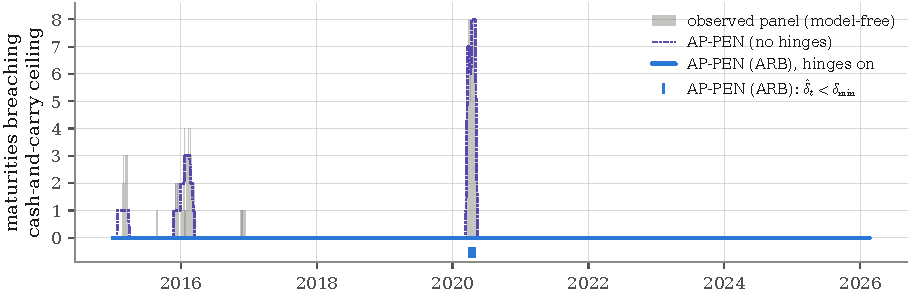
\includegraphics[width=0.87\textwidth]{figures/results/real3_constraint_activity.pdf}
        \caption{Cash-and-carry ceiling breaches by date. The model-free shaded series is computed directly from observables $(F^{\mathrm{obs}}, S_t, \tau, r_t)$. The thick blue line, AP-PEN (ARB) with the hinge losses switched on, sits exactly at zero across the entire sample: enforcing the cash-and-carry hinge means the model never breaches the ceiling, so its breach count is identically zero throughout, unlike the unconstrained variant (violet, dash-dot), which tracks the observed breaches closely. The small blue marker beneath the axis, near 2020, flags the separate dates on which AP-PEN (ARB)'s recovered $\hat{\delta}_t$ itself falls below the convenience-yield floor $\delta_{\min}$; this is a statement about the latent state rather than about price breaches, so it is shown as a rug below the axis rather than as a curve sharing the $y$-axis units.}
        \label{fig:constraint_activity}
    \end{subfigure}

    \vspace{0.5cm}

    \begin{subfigure}{\textwidth}
        \centering
        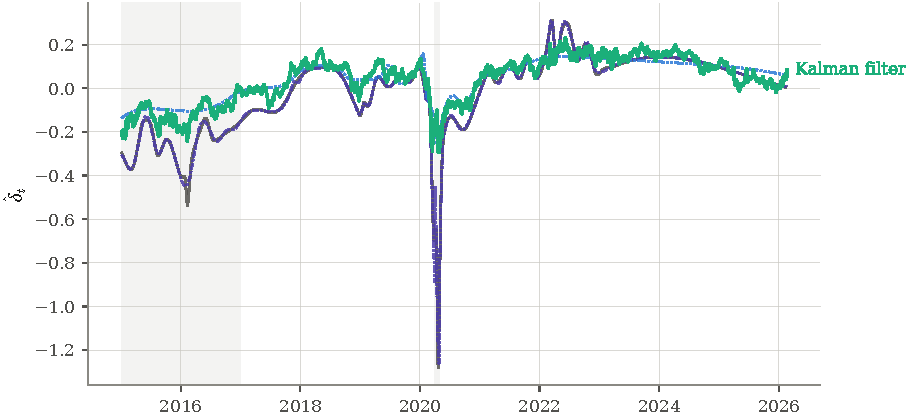
\includegraphics[width=0.87\textwidth]{figures/results/real2_pinn_vs_kalman.pdf}
        \caption{Recovered $\hat{\delta}_t$ across model variants compared against the benchmark KF path.}
        \label{fig:real2_pinn_vs_kalman}
    \end{subfigure}

    \caption{Constraint activity (a) and recovered convenience-yield paths (b) for the WTI panel (2015--2026). In (a), raw market breaches occur in $1.84\%$ of points, clustered during the 2015--2016 shale glut and April 2020 dislocations. Unconstrained AP-PEN mirrors these breaches ($2.00\%$), whereas AP-PEN (ARB) eliminates them entirely ($0.00\%$). In (b), unconstrained models diverge to implausible extremes below $-1.2$ in April 2020, while AP-PEN (ARB) preserves economically plausible bounds.}
    \Description{Two stacked panels: cash-and-carry constraint breaches by date for each model variant, and the recovered convenience-yield paths of each variant against the Kalman filter benchmark.}
    \label{fig:real_results_combined}
\end{figure*}

The magnitude of this divergence is best understood through the GS economic dynamics. Unlike CIR-style models~\cite{Liu2009No-ArbitrageStructures} that enforce $\delta \ge 0$ by construction, the Ornstein--Uhlenbeck process~\cite{uhlenbeck1930theory} is unbounded. Section~\ref{sec:pinn_inversion} deliberately avoids imposing an idealised non-negativity floor on $\hat{\delta}_t$ because deep-contango regimes, like the one experienced in April 2020, actively produce negative convenience yields. The KF baseline confirmed this architectural choice, with its own recovered $\hat{\delta}_t$ dipping to $-0.293$ during that same period. Conversely, the unconstrained variants overshoot by roughly an order of magnitude, with the vanilla AP-PEN and MLP models recovering $-1.26$ and $-1.28$ respectively, and the closed-form LS reaching $-1.65$. This suggests they are not simply finding a more extreme answer, but capturing a different phenomenon entirely. The economic literature supports this: the April 2020 WTI anomaly was driven by logistical factors (specifically a demand shock, oversupply, and a physical storage shortage at the Cushing delivery hub~\cite{Burns2022Arbitrage}) rather than a fundamental repricing of the value of holding oil. Notably, Brent crude, which shares WTI's convenience-yield economics but lacks its Cushing-specific delivery obligations, never went negative~\cite{FernandezPerez2022Negative}. Ultimately, the unconstrained variants appear to improperly absorb a localised market-microstructure event into a state variable never designed to carry it.

The necessity of physical guardrails to prevent this absorption is evident in the activity of the inequality constraints (Fig.~\ref{fig:constraint_activity}). On the observed panel, the raw data violates the cash-and-carry ceiling on $1.84\%$ of the $22{,}160$ points (across $135$ dates), primarily concentrated during the 2015--2016 shale glut and the 2020 storage-exhaustion events~\cite{fattouh2016oilfall, gilje2024benchmarks}. Attempting to faithfully fit this data, the unconstrained variants (MLP, vanilla AP-PEN) slightly amplify the error, yielding violation rates of $1.98\%$ and $2.00\%$. Once the constraints are activated in AP-PEN (ARB), cash-and-carry violations drop to exactly zero, and violations of the convenience-yield floor fall from roughly $7\%$ to $0.69\%$. Whether a constraint earns its keep is therefore decidable in advance: the violation rate is computable directly from the observed quantities $(F^{\mathrm{obs}}, S_t, \tau, r_t)$ before any model is fitted. On real-market data, the guardrails clearly justify their inclusion, but only because the underlying data violates them. Because the squared hinge loss has zero gradient wherever a bound is already satisfied, market conditions with no violations would render the no-arbitrage variant identical to its unconstrained twin. Furthermore, because the reverse cash-and-carry constraint is never triggered for any model, only two of the three hinge terms actively shape the $\delta_t$ recovery.

\begin{table}[tbp]
\centering
\footnotesize
\caption{Recovered structural parameters on real WTI. KF is the
full-sample MLE (\S\ref{sec:kalman}); Closed-form LS is the profiled MLE of
\S\ref{sec:ls_baseline}, estimating only the identified coordinates. The
$\kappa$ floor is shown only for AP-PEN (ARB), the variant it binds on
(\S\ref{sec:pinn_inversion}). Only the top block is identified from a futures
panel (\S\ref{sec:identifiability}); place no economic reading on the lower
block.}
\label{tab:real_psi_pathology}
\resizebox{\columnwidth}{!}{%
\begin{tabular}{lrrrrr}
\toprule
& & & & \multicolumn{2}{c}{AP-PEN (ARB)} \\
\cmidrule(lr){5-6}
Parameter & KF (MLE) & Closed-form LS & AP-PEN & unfloored & $\kappa_{\min}=0.1$ \\
\midrule
$\kappa$      & $0.4257$ & $0.9512$ & $0.9301$ & $0.0028$ & $0.1002$ \\
$\sigma_2$    & $0.1726$ & $0.5516$ & $0.5444$ & $0.0557$ & $0.0481$ \\
$m$           & $0.0811$ & $0.1871$ & $0.1888$ & $-4.5436$ & $-0.0206$ \\
\midrule
$\sigma_1$    & $0.4397$ & --- & $0.7660$ & $0.0051$ & $0.0031$ \\
$\rho$        & $0.8883$ & --- & $0.9676$ & $-0.8198$ & $-0.0188$ \\
$\alpha^{\mathbb{Q}}$ & $-0.0773$ & --- & $-0.2450$ & $-4.4599$ & $-0.0206$ \\
$\alpha^{\mathbb{P}}$ & $0.1007$ & --- & $0.0120$ & $4.3741$ & $0.1900$ \\
\bottomrule
\end{tabular}%
}
\end{table}

Although Table~\ref{tab:real_kalman_comparison} shows strong path recovery for AP-PEN (ARB), Table~\ref{tab:real_psi_pathology} reveals severe underlying parameter pathologies, mirroring synthetic findings and the theoretical limits predicted in \S\ref{sec:identifiability}. When the hinge loss terms are active without parameter bounds, the mean-reversion speed $\kappa$ collapses to near zero ($0.0028$). Spot volatility $\sigma_1$ ($0.0051$) and correlation $\rho$ ($-0.8198$) also collapse, with a negative $\rho$ relative to every other calibration. While individual unidentifiable parameters carry little stand-alone meaning (\S\ref{sec:identifiability}), the simultaneous collapse of $\kappa$, $\sigma_1$, $\rho$, $\alpha^{\mathbb{Q}}$ ($-4.46$), and $m$ ($-4.54$) diagnoses a structural failure mode rather than arbitrary convergence among equivalent solutions. Imposing a lower bound $\kappa_{\min}=0.1$ causes the model to converge exactly onto the floor across five random restarts ($\kappa = 0.100 \pm 0.000$), confirming that the constraint mechanism drives this degeneracy rather than stochastic variation. Ultimately, AP-PEN (ARB) achieves the strongest KF $\delta_t$ recovery only by pushing parameters into a degenerate state, while pinning its recovered path directly against the lower boundary ($\hat{\delta}_t = -0.301 \approx \delta_{\min} = -0.30$) rather than finding a genuinely superior economic solution.



\section{Future Work}
\label{sec:future_work}
The work presented here offers several avenues to extend and modify AP-PEN. A natural next step would be to analyse the model's performance out-of-sample to evaluate if its $\delta$ recovery generalises to future time-frames. Second to this, adapting the architecture to non-affine commodity models lacking closed-form solutions, such as the state-dependent volatility framework by Trolle--Schwartz~\cite{chen2017pricing} and the $3/2$ model~\cite{kouarfate2021explicit}, would be meaningful and important extensions. Because both account for stochastic volatility alongside convenience yields, their PDE residuals serve as direct commodity analogues to the Dupire model used in WamOL~\cite{Hoshisashi2024Whack-a-moleSurface, dupire1994pricing}, re-introducing the PINN machinery that was removed for this use case. Additionally, integrating Fourier-feature embeddings could improve AP-PEN's capacity to capture fine-scale variance in convenience-yield dynamics~\cite{tancik2020fourier}. Finally, the commodity-specific no-arbitrage and economic constraint losses developed here could be extended to include genuine derivative-constraint terms mirroring~\cite{Hoshisashi2024Physics-InformedPDEs} to govern the shape of the forward curve, alongside targeted loss constraints on the volatility surfaces of the proposed model extensions.

Broadly, accurate and timely commodity pricing propagates through supply chains, energy security, and food prices, ultimately impacting consumers worldwide. This work lays the foundation for developing efficient modern approaches to estimate latent states in commodity markets, enabling optimal inventory and resource allocation at a fraction of the current computational cost. Furthermore, while such estimators have historically been restricted to large institutions with vast compute, this framework democratises that capability for smaller market participants.


%% ════════════════════════════════════════════════════════════════════════════
%% 6. CONCLUSION 
%% ════════════════════════════════════════════════════════════════════════════
\section{Conclusion}
\label{sec:conclusion}
This thesis has presented a constrained, physics-enforced model for recovering the latent convenience yield from real futures data. The partitioning of the affine structure recovers the convenience yield reliably and accurately identifies several parameters of $\psi$, but it cannot separate $\sigma_1$ from $\rho$. On the arbitrage-free synthetic data panel, the economic constraints imposed on the network are counterproductive, but they are materially useful on real data. On both data panels, there was an orthogonal relationship between the success of $\psi$ and $\delta$ recovery.

The primary contribution of this thesis has been the extension of the WamOL and DC-PINN frameworks to the domain of commodities with an identification analysis and a constrained latent-path estimator benchmarked against the incumbent method (KF), rather than a novel extension of the classical PINN architecture to recover the risk premia. This is in fact one of the main limitations of this architecture. The affine nature of the GS model used in this design prevented the use of the PDE residual, a hallmark of Raissi-style PINNs~\cite{Raissi2019Physics-informedEquations}. Therefore, any \textit{physics} had to be enforced by construction rather than learned. This approach was necessary to allow the use of the economic constraints, which proved successful at constraining the model's outputs on real-world data, a capability unavailable to the simple LS approach.

The results of this study prove the validity and usefulness of novel commodity-specific economic constraints and thus the generalisation of WamOL to commodity markets, while at the same time revealing limitations in modelling affine models. Finally, the importance of convenience yield must be emphasised. For crude oil, it represents a deliberate strategic representation of inventory scarcity~\cite{Gibson1990StochasticClaims} and as such, a model that recovers it reliably, even where the underlying structural parameters remain unidentifiable, already delivers the quantity that matters most for risk management and storage decisions in practice.

\begin{acks}
I sincerely thank my supervisors, Dr. Lama Hamadeh and Dr. Carolyn Phelan, for their continuous guidance and vital feedback throughout the research and writing of this thesis. I am also deeply grateful to Dr. Kentaro Hoshisashi, a valued advisor whose work directly inspired my own. Finally, I thank my family for their unwavering support throughout my Master's degree; without them, this experience would not have been possible.
\end{acks}

\bibliographystyle{ACM-Reference-Format}
\bibliography{references}


%% ════════════════════════════════════════════════════════════════════════════
%% APPENDICES
%% ════════════════════════════════════════════════════════════════════════════
\appendix

\section{Code}
The project code is available on GitHub:~\url{https://github.com/Metahemeralism/AP-PEN}





\section{Derivation of the Futures Pricing PDE and Closed Form}
\label{app:gs_pde}

This appendix derives the futures pricing PDE (Eq.~\ref{eq:gs_pde_tau}) from the risk-neutral dynamics, transforms it to time-to-maturity, and obtains the closed-form exponential-affine solution of Eqs.~\ref{eq:gs_futures}--\ref{eq:app_A}.

\subsection{It\^{o}'s lemma and the futures PDE}

Let $F = F(S_t, \convyield_t, t)$ be the futures price. By the bivariate It\^{o} lemma,
\begin{equation}
  \label{eq:app_ito}
  \begin{multlined}
  \mathrm{d}F = \frac{\partial F}{\partial t}\,\mathrm{d}t
    + \frac{\partial F}{\partial S}\,\mathrm{d}S_t
    + \frac{\partial F}{\partial \convyield}\,\mathrm{d}\convyield_t \\
    + \frac{1}{2}\frac{\partial^2 F}{\partial S^2}(\mathrm{d}S_t)^2
    + \frac{\partial^2 F}{\partial S\,\partial \convyield}(\mathrm{d}S_t)(\mathrm{d}\convyield_t) \\
    + \frac{1}{2}\frac{\partial^2 F}{\partial \convyield^2}(\mathrm{d}\convyield_t)^2.
  \end{multlined}
\end{equation}
\noindent
The quadratic-variation terms, with $\mathrm{d}W_1^{\mathbb{Q}}\,\mathrm{d}W_2^{\mathbb{Q}} = \rho\,\mathrm{d}t$, are
\begin{equation}
  \label{eq:app_qv}
  \begin{gathered}
  (\mathrm{d}S_t)^2 = \sigma_1^2 S_t^2\,\mathrm{d}t,
  \qquad
  (\mathrm{d}\convyield_t)^2 = \sigma_2^2\,\mathrm{d}t, \\
  (\mathrm{d}S_t)(\mathrm{d}\convyield_t) = \rho\,\sigma_1\sigma_2 S_t\,\mathrm{d}t.
  \end{gathered}
\end{equation}
\noindent
Substituting the $\mathbb{Q}$-dynamics (Eqs.~\ref{eq:app_spot_Q}, \ref{eq:app_cy_Q}) and collecting the drift,
\begin{equation}
  \label{eq:app_dF}
  \begin{aligned}
  \mathrm{d}F = \Bigg[
    &\frac{\partial F}{\partial t}
    + (r - \convyield_t)S_t\frac{\partial F}{\partial S} \\
    &+ \meanrev(\longrun^{\mathbb{Q}} - \convyield_t)\frac{\partial F}{\partial \convyield}
    + \frac{1}{2}\sigma_1^2 S_t^2\frac{\partial^2 F}{\partial S^2} \\
    &+ \rho\sigma_1\sigma_2 S_t\frac{\partial^2 F}{\partial S\,\partial \convyield}
    + \frac{1}{2}\sigma_2^2\frac{\partial^2 F}{\partial \convyield^2}
  \Bigg]\mathrm{d}t \\
  &+ \sigma_1 S_t\frac{\partial F}{\partial S}\,\mathrm{d}W_1^{\mathbb{Q}}
  + \sigma_2\frac{\partial F}{\partial \convyield}\,\mathrm{d}W_2^{\mathbb{Q}}.
  \end{aligned}
\end{equation}
\noindent
A futures contract requires no initial investment, so $F$ must be a $\mathbb{Q}$-martingale: its drift vanishes, $\mathbb{E}^{\mathbb{Q}}[\mathrm{d}F] = 0$. Setting the bracket to zero gives the GS PDE,
\begin{equation}
  \label{eq:app_pde_calendar}
  \begin{multlined}
  \frac{\partial F}{\partial t}
  + (r - \convyield)S\frac{\partial F}{\partial S}
  + \meanrev(\longrun^{\mathbb{Q}} - \convyield)\frac{\partial F}{\partial \convyield} \\
  + \frac{1}{2}\sigma_1^2 S^2\frac{\partial^2 F}{\partial S^2}
  + \rho\sigma_1\sigma_2 S\frac{\partial^2 F}{\partial S\,\partial \convyield} \\
  + \frac{1}{2}\sigma_2^2\frac{\partial^2 F}{\partial \convyield^2} = 0,
  \end{multlined}
\end{equation}
\noindent
subject to the terminal condition $F(S, \convyield, T) = S$.

\subsection{Change of variables: time-to-maturity}

In calendar time the terminal condition sits at $t = T$, which differs across contracts, undesirable for a network learning a single function valid across all maturities. Re-expressing in time-to-maturity $\tau = T - t$ collapses the terminal condition to the fixed point $\tau = 0$.

Let $\hat{F}(S, \convyield, \tau) := F(S, \convyield, t)$. Since $t = T - \tau$, the chain rule gives $\partial t/\partial \tau = -1$, so
\begin{equation}
  \label{eq:app_chain}
  \frac{\partial F}{\partial t} = -\frac{\partial \hat{F}}{\partial \tau}.
\end{equation}
\noindent
The spatial derivatives are unchanged, since $S$ and $\convyield$ depend on neither $t$ nor $\tau$. Substituting Eq.~\ref{eq:app_chain} into Eq.~\ref{eq:app_pde_calendar} and rearranging yields a forward equation in $\tau$,
\begin{equation}
  \label{eq:app_pde_tau}
  \begin{multlined}
  \frac{\partial \hat{F}}{\partial \tau}
  = (r - \convyield)S\frac{\partial \hat{F}}{\partial S}
  + \meanrev(\longrun^{\mathbb{Q}} - \convyield)\frac{\partial \hat{F}}{\partial \convyield} \\
  + \frac{1}{2}\sigma_1^2 S^2\frac{\partial^2 \hat{F}}{\partial S^2}
  + \rho\sigma_1\sigma_2 S\frac{\partial^2 \hat{F}}{\partial S\,\partial \convyield} \\
  + \frac{1}{2}\sigma_2^2\frac{\partial^2 \hat{F}}{\partial \convyield^2},
  \end{multlined}
\end{equation}
\noindent
with the terminal condition becoming an initial condition,
\begin{equation}
  \label{eq:app_ic}
  \hat{F}(S, \convyield, 0) = S.
\end{equation}
\noindent
This is a well-posed initial value problem in $\tau$ alone, which is the form imposed directly in the pricing transform (\S\ref{sec:pinn_inversion}) rather than solved by collocation; $\tau$ is the interval between each observation date and the contract's delivery date.

\subsection{Closed-form solution}

Equation~\ref{eq:app_pde_tau} with $\hat{F}(S, \convyield, 0) = S$ admits a closed-form, exponential-affine solution. Take the ansatz
\begin{equation}
  \label{eq:app_ansatz}
  \hat{F}(S, \convyield, \tau) = S\exp\!\big(B(\tau)\convyield + A(\tau)\big),
\end{equation}
\noindent
whose derivatives are
\begin{equation}
  \label{eq:app_derivs}
  \begin{gathered}
  \frac{\partial \hat{F}}{\partial S} = \frac{\hat{F}}{S},
  \qquad
  \frac{\partial^2 \hat{F}}{\partial S^2} = 0,
  \qquad
  \frac{\partial \hat{F}}{\partial \convyield} = B\hat{F}, \\
  \frac{\partial^2 \hat{F}}{\partial \convyield^2} = B^2\hat{F},
  \qquad
  \frac{\partial^2 \hat{F}}{\partial S\,\partial \convyield} = B\frac{\hat{F}}{S}, \\
  \frac{\partial \hat{F}}{\partial \tau} = \hat{F}\big(B'\convyield + A'\big).
  \end{gathered}
\end{equation}
\noindent
Inserting these into Eq.~\ref{eq:app_pde_tau} and dividing through by $\hat{F}$,
\begin{equation}
  \label{eq:app_substituted}
  B'\convyield + A'
  = (r - \convyield)
  + \meanrev(\longrun^{\mathbb{Q}} - \convyield)B
  + \rho\sigma_1\sigma_2 B
  + \frac{1}{2}\sigma_2^2 B^2.
\end{equation}
\noindent
The $\tfrac{1}{2}\sigma_1^2 S^2\,\partial^2\hat{F}/\partial S^2$ term vanishes since $\hat{F}_{SS} = 0$ for the ansatz. Matching the coefficient of $\convyield$ and the constant term gives two decoupled ODEs with $B(0) = A(0) = 0$:
\begin{align}
  \label{eq:app_ode_B}
  B'(\tau) &= -1 - \meanrev B(\tau), \\
  \label{eq:app_ode_A}
  A'(\tau) &= r + \big(\meanrev\longrun^{\mathbb{Q}} + \rho\sigma_1\sigma_2\big)B(\tau) + \frac{1}{2}\sigma_2^2 B(\tau)^2.
\end{align}

\paragraph{Solving for $B(\tau)$.} The linear ODE $B' + \meanrev B = -1$ has integrating factor $e^{\meanrev\tau}$, giving $e^{\meanrev\tau}B = -\tfrac{1}{\meanrev}e^{\meanrev\tau} - C$. Applying $B(0) = 0$ fixes $C = -\tfrac{1}{\meanrev}$, so
\begin{equation}
  \label{eq:app_B}
  B(\tau) = -\frac{1 - e^{-\meanrev\tau}}{\meanrev}.
\end{equation}

\paragraph{Solving for $A(\tau)$.} Squaring,
\begin{equation}
  \label{eq:app_Bsq}
  B(\tau)^2 = \frac{1 - 2e^{-\meanrev\tau} + e^{-2\meanrev\tau}}{\meanrev^2};
\end{equation}
\noindent
the $e^{-2\meanrev\tau}$ term is the source of the second exponential below. Substituting $B$ and $B^2$ into Eq.~\ref{eq:app_ode_A} and integrating term by term from $0$ to $\tau$ with $A(0) = 0$,
\begin{equation}
  \label{eq:app_A}
  \begin{multlined}
  A(\tau) = \left(r - \longrun^{\mathbb{Q}} + \frac{1}{2}\frac{\sigma_2^2}{\meanrev^2} - \frac{\sigma_1\sigma_2\rho}{\meanrev}\right)\tau \\
  + \frac{1}{4}\sigma_2^2\frac{1 - e^{-2\meanrev\tau}}{\meanrev^3} \\
  + \left(\longrun^{\mathbb{Q}}\meanrev + \sigma_1\sigma_2\rho - \frac{\sigma_2^2}{\meanrev}\right)\frac{1 - e^{-\meanrev\tau}}{\meanrev^2}.
  \end{multlined}
\end{equation}

\paragraph{Result.} Collecting,
\begin{equation}
  \label{eq:app_result}
  \begin{gathered}
  \hat{F}(S, \convyield, \tau) = S\exp\!\big(B(\tau)\convyield + A(\tau)\big), \\
  B(\tau) = -\frac{1 - e^{-\meanrev\tau}}{\meanrev},
  \end{gathered}
\end{equation}
\noindent
with $A(\tau)$ as in Eq.~\ref{eq:app_A}. These are Eqs.~\ref{eq:gs_futures} and~\ref{eq:app_A}, and match the Schwartz (1997) Model~2 closed form term by term under the identification $\longrun^{\mathbb{Q}} = \longrun^{\mathbb{P}} - \sigma_2\lambda_2/\meanrev$, with his maturity $T$ playing the role of $\tau$.



\section{Change of Measure: Physical to Risk-Neutral Dynamics}
\label{app:gs_derivation}

This appendix derives the risk-neutral system of Eqs.~\ref{eq:gs_spot}--\ref{eq:gs_cy} from the physical dynamics, pinning down the two market prices of risk and showing that only the long-run convenience-yield level is shifted by the change of measure.

\subsection{Physical dynamics}

Work on a filtered probability space $(\Omega, \mathcal{F}, \{\mathcal{F}_t\}_{t\geq 0}, \mathbb{P})$. Under the physical measure $\mathbb{P}$, the spot price $S_t$ and convenience yield $\convyield_t$ evolve as
\begin{align}
  \label{eq:app_spot_P}
  \mathrm{d}S_t &= (\mu - \convyield_t)\,S_t\,\mathrm{d}t + \sigma_1 S_t\,\mathrm{d}W_1^{\mathbb{P}}, \\
  \label{eq:app_cy_P}
  \mathrm{d}\convyield_t &= \meanrev(\longrun^{\mathbb{P}} - \convyield_t)\,\mathrm{d}t + \sigma_2\,\mathrm{d}W_2^{\mathbb{P}},
\end{align}
\noindent
with correlated drivers $\mathrm{d}W_1^{\mathbb{P}}\,\mathrm{d}W_2^{\mathbb{P}} = \rho\,\mathrm{d}t$, $\rho \in (-1, 1)$. Here $\mu$ is the total expected return on the commodity: the price-appreciation drift is $(\mu - \convyield_t)$, with the convenience yield $\convyield_t$ acting as the continuous dividend-analogue benefit of holding physical inventory.

\subsection{Girsanov change of measure}

Under the risk-neutral measure $\mathbb{Q}$, traded assets must drift at the risk-free rate $r$. We introduce a market price of risk $\lambda_i$ for each Brownian driver. By Girsanov's theorem,
\begin{equation}
  \label{eq:app_girsanov}
  \mathrm{d}W_i^{\mathbb{Q}} = \mathrm{d}W_i^{\mathbb{P}} + \lambda_i\,\mathrm{d}t, \qquad i = 1, 2,
\end{equation}
\noindent
with the measure change defined by the Radon--Nikod\'ym derivative
\begin{equation}
  \label{eq:app_rn}
  \begin{multlined}
  \left.\frac{\mathrm{d}\mathbb{Q}}{\mathrm{d}\mathbb{P}}\right|_{\mathcal{F}_t}
  = \exp\!\Bigg(
    -\int_0^t \lambda_1\,\mathrm{d}W_1^{\mathbb{P}}
    -\int_0^t \lambda_2\,\mathrm{d}W_2^{\mathbb{P}} \\
    -\frac{1}{2}\int_0^t \big(\lambda_1^2 + \lambda_2^2\big)\,\mathrm{d}s
  \Bigg).
  \end{multlined}
\end{equation}
\noindent
Rearranging Eq.~\ref{eq:app_girsanov} gives $\mathrm{d}W_i^{\mathbb{P}} = \mathrm{d}W_i^{\mathbb{Q}} - \lambda_i\,\mathrm{d}t$. Substituting into Eqs.~\ref{eq:app_spot_P}--\ref{eq:app_cy_P},
\begin{align}
  \label{eq:app_spot_sub}
  \mathrm{d}S_t &= \big[(\mu - \convyield_t) - \sigma_1\lambda_1\big] S_t\,\mathrm{d}t + \sigma_1 S_t\,\mathrm{d}W_1^{\mathbb{Q}}, \\
  \label{eq:app_cy_sub}
  \begin{split}
  \mathrm{d}\convyield_t &= \big(\meanrev\longrun^{\mathbb{P}} - \sigma_2\lambda_2 - \meanrev\convyield_t\big)\,\mathrm{d}t \\
    &\quad + \sigma_2\,\mathrm{d}W_2^{\mathbb{Q}}.
  \end{split}
\end{align}
\noindent
These are correct but leave $\lambda_1, \lambda_2$ unspecified, and the convenience-yield drift is no longer in mean-reverting form. We resolve each in turn.

\subsection{Pinning down \texorpdfstring{$\lambda_1$}{lambda1}: the no-arbitrage drift condition}

The economic content of no-arbitrage here is the cost-of-carry condition. Over an instant $\mathrm{d}t$, a holder of one unit of the physical commodity earns its price appreciation $(\mu - \convyield_t)$ plus the convenience yield $\convyield_t$, the non-pecuniary benefit of holding inventory (avoiding stock-outs, retaining operational flexibility). These sum to the total expected return $\mu$.
\noindent
Imposing the risk-neutral price drift on Eq.~\ref{eq:app_spot_sub}, the spot, as a traded asset paying continuous convenience yield $\convyield_t$, must have price drift $(r - \convyield_t)$. Matching,
\begin{equation}
  \label{eq:app_lambda1}
  (\mu - \convyield_t) - \sigma_1\lambda_1 = r - \convyield_t
  \quad\Longrightarrow\quad
  \lambda_1 = \frac{\mu - r}{\sigma_1},
\end{equation}
\noindent
which identifies $\lambda_1$ as the Sharpe ratio of the spot process. Substituting back,
\begin{equation}
  \label{eq:app_spot_Q}
  \mathrm{d}S_t = (r - \convyield_t)\,S_t\,\mathrm{d}t + \sigma_1 S_t\,\mathrm{d}W_1^{\mathbb{Q}},
\end{equation}
\noindent
recovering Eq.~\ref{eq:gs_spot}.

\subsection{Pinning down \texorpdfstring{$\longrun^{\mathbb{Q}}$}{alphaQ}: restoring mean-reverting form}

Factoring $\meanrev$ back out of the drift in Eq.~\ref{eq:app_cy_sub},
\begin{equation}
  \label{eq:app_alphaQ}
  \begin{split}
  \meanrev\longrun^{\mathbb{P}} - \sigma_2\lambda_2
  &= \meanrev\!\left(\longrun^{\mathbb{P}} - \frac{\sigma_2\lambda_2}{\meanrev}\right) \\
  &=: \meanrev\longrun^{\mathbb{Q}}.
  \end{split}
\end{equation}
\noindent
Unlike $\lambda_1$, the convenience-yield risk premium $\lambda_2$ is not fixed by a no-arbitrage argument, since $\convyield_t$ is not a traded asset; it is identified jointly with the other parameters by calibration to the observed futures term structure. Substituting back,
\begin{equation}
  \label{eq:app_cy_Q}
  \begin{gathered}
  \mathrm{d}\convyield_t = \meanrev(\longrun^{\mathbb{Q}} - \convyield_t)\,\mathrm{d}t + \sigma_2\,\mathrm{d}W_2^{\mathbb{Q}}, \\
  \longrun^{\mathbb{Q}} = \longrun^{\mathbb{P}} - \frac{\sigma_2\lambda_2}{\meanrev},
  \end{gathered}
\end{equation}
\noindent
recovering Eq.~\ref{eq:gs_cy}. Only the long-run level shifts, $\longrun^{\mathbb{P}} \to \longrun^{\mathbb{Q}}$; the mean-reversion speed $\meanrev$ and volatility $\sigma_2$ are unchanged. This completes the derivation of the risk-neutral system used throughout \S\ref{sec:gs_model}.

\section{Supplementary Results}
\label{app:supplementary}

\paragraph{Half-life, identifiability floor, and softplus parameterisation.}
Under the OU dynamics
\[
d\delta_t=\kappa(\alpha-\delta_t)\,dt+\sigma_2\,dW_t,
\]
the conditional mean decays as
\[
\mathbb{E}[\delta_t-\alpha\mid \delta_0]=(\delta_0-\alpha)e^{-\kappa t}.
\]
Define the half-life \(t_{1/2}\) by
\[
e^{-\kappa t_{1/2}}=\tfrac12
\quad\Rightarrow\quad
t_{1/2}=\frac{\ln 2}{\kappa}.
\]

For futures loading
\[
B(\tau)=-\frac{1-e^{-\kappa\tau}}{\kappa},
\]
if \(\kappa\tau\ll 1\), then \(B(\tau)\approx-\tau\), so curvature in \(\tau\) (which identifies \(\kappa\)) is weak.  
With \(\tau_{\max}=1.88\) years and \(\kappa\le 0.1\), we have
\[
t_{1/2}\ge \frac{\ln 2}{0.1}=6.93\ \text{years}\gg 1.88,
\]
so over observed maturities the loading is nearly linear and \(\kappa\) is poorly identified.  
Hence we impose \(\kappa_{\min}=0.1\) to exclude this structurally uninformative region.

We enforce this smoothly via
\[
\kappa=\kappa_{\min}+\operatorname{softplus}(\theta),\qquad \kappa_{\min}=0.1,
\]
which guarantees \(\kappa\ge 0.1\) while preserving unconstrained optimisation in \(\theta\).

%% Authored at 2.80in each. At 0.49\columnwidth (1.63in) they rendered at
%% 0.58x, taking their 9pt labels to ~5pt. Spanning at 0.40\textwidth = 2.80in
%% is exactly 1.00x, and 2 wide x 3 tall fits inside one spanning float.
\begin{figure*}[tp]
    \centering
    \begin{subfigure}[b]{0.40\textwidth}
        \centering
        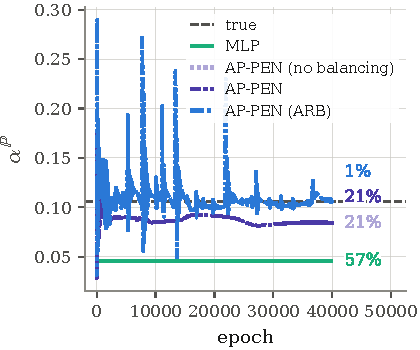
\includegraphics[width=\linewidth]{figures/results/pinn1_alphaP.pdf}
        \caption{$\alpha^{\mathbb{P}}$ recovery}
        \label{fig:pinn1_alphaP}
    \end{subfigure}\hfill
    \begin{subfigure}[b]{0.40\textwidth}
        \centering
        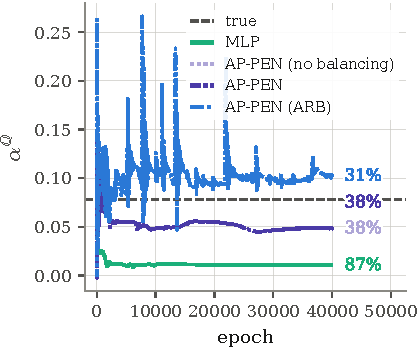
\includegraphics[width=\linewidth]{figures/results/pinn1_alphaQ.pdf}
        \caption{$\alpha^{\mathbb{Q}}$ recovery}
        \label{fig:pinn1_alphaQ}
    \end{subfigure}

    \vspace{0.3cm}

    \begin{subfigure}[b]{0.40\textwidth}
        \centering
        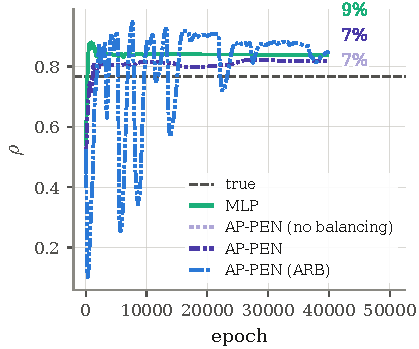
\includegraphics[width=\linewidth]{figures/results/pinn1_rho.pdf}
        \caption{$\rho$ recovery}
        \label{fig:pinn1_rho}
    \end{subfigure}\hfill
    \begin{subfigure}[b]{0.40\textwidth}
        \centering
        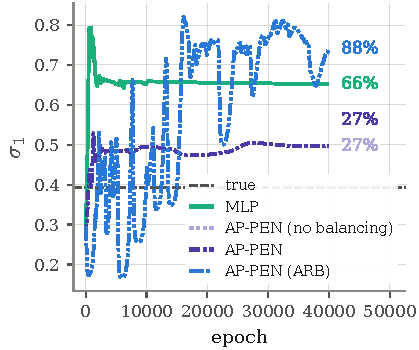
\includegraphics[width=\linewidth]{figures/results/pinn1_sigma1.pdf}
        \caption{$\sigma_1$ recovery}
        \label{fig:pinn1_sigma1}
    \end{subfigure}

    \vspace{0.3cm}

    \begin{subfigure}[b]{0.40\textwidth}
        \centering
        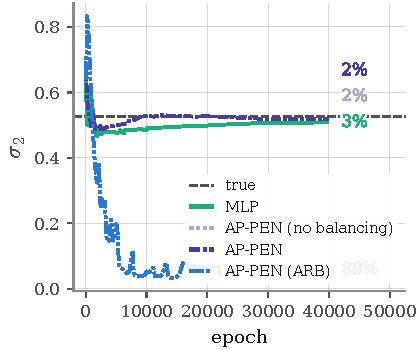
\includegraphics[width=\linewidth]{figures/results/pinn1_sigma2.pdf}
        \caption{$\sigma_2$ recovery}
        \label{fig:pinn1_sigma2}
    \end{subfigure}\hfill
    \begin{subfigure}[b]{0.40\textwidth}
        \centering
        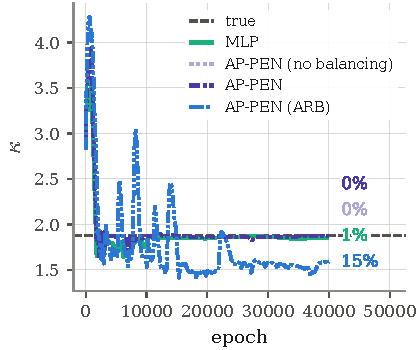
\includegraphics[width=\linewidth]{figures/results/pinn1_kappa.pdf}
        \caption{$\kappa$ recovery}
        \label{fig:pinn1_kappa}
    \end{subfigure}

    \caption{Per-parameter recovery across variants over 40k training epochs,
    synthetic panel. Referenced from \S\ref{sec:synthetic}: the identified
    coordinates ($\kappa$, $\sigma_2$) converge tightly to their true values
    (dashed), while $\alpha^{\mathbb{P}}$, $\alpha^{\mathbb{Q}}$, $\rho$ and
    $\sigma_1$ do not, consistent with the identifiability result of
    \S\ref{sec:identifiability}. Percentages give each variant's final
    relative error against the true value.}
    \Description{Six line plots showing the recovery of each structural parameter across training epochs for every model variant, against the true value.}
    \label{fig:param_recovery_appendix}
\end{figure*}

\subsection{Training Loss Convergence}
\label{sec:training_convergence}

%% Authored at 6.07in. At 0.85\columnwidth (2.83in) these rendered at 0.47x --
%% 9pt axis labels down to ~4pt. They have to span: 0.87\textwidth = 6.09in is
%% 1.00x. Stacked rather than three-across for the same reason.
\begin{figure*}[tp]
    \centering
    \begin{subfigure}[b]{0.87\textwidth}
        \centering
        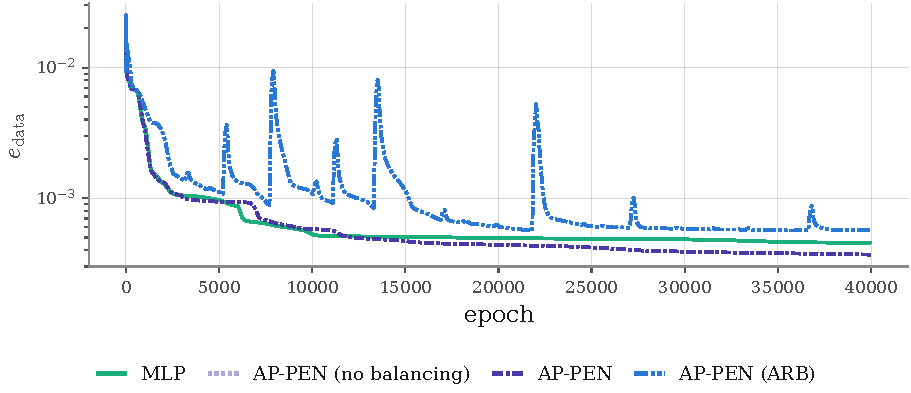
\includegraphics[width=\linewidth]{figures/results/pinn0a_training_data.pdf}
        \caption{Data misfit loss}
        \label{fig:pinn0a_training_data}
    \end{subfigure}

    \vspace{0.25cm}

    \begin{subfigure}[b]{0.87\textwidth}
        \centering
        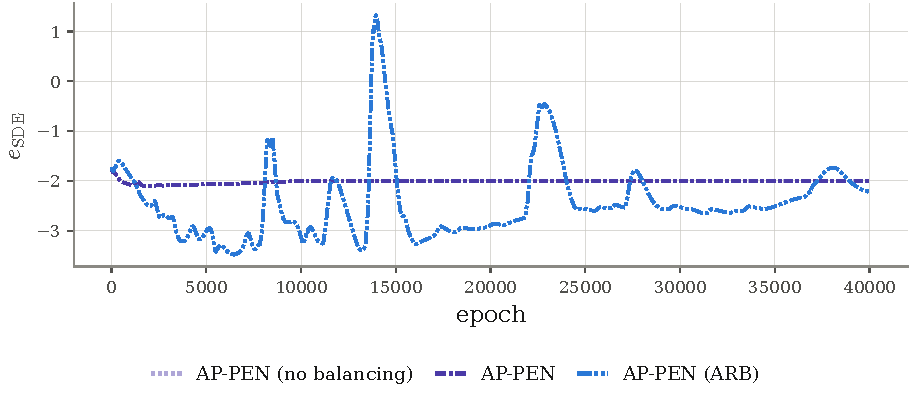
\includegraphics[width=\linewidth]{figures/results/pinn0b_training_sde.pdf}
        \caption{SDE transition NLL}
        \label{fig:pinn0b_training_sde}
    \end{subfigure}

    \vspace{0.25cm}

    \begin{subfigure}[b]{0.87\textwidth}
        \centering
        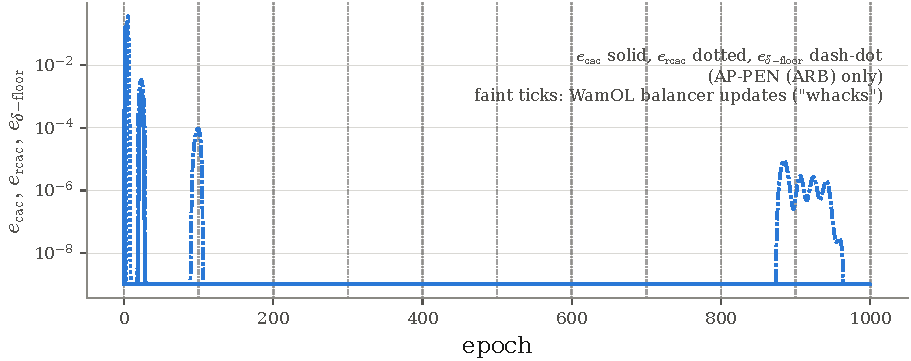
\includegraphics[width=\linewidth]{figures/results/pinn0c_training_hinges.pdf}
        \caption{Hinge losses (ARB)}
        \label{fig:pinn0c_training_hinges}
    \end{subfigure}

    \caption{Training loss convergence across variants. In (c), faint dotted
    vertical lines mark the WamOL loss-balancer's gradient-norm reweighting
    updates (the ``whacks'' of Whack-a-mole Online Learning~\cite{Hoshisashi2024Whack-a-moleSurface}),
    which recur every $100$ epochs for AP-PEN (ARB); each hinge-loss transient
    coincides with several such updates. Per-parameter recovery curves for
    the same runs are in Appendix~\ref{app:supplementary},
    Fig.~\ref{fig:param_recovery_appendix}.}
    \Description{Three line plots of training loss against epoch for the data-misfit, SDE-transition and hinge loss channels across model variants.}
    \label{fig:training_losses}
\end{figure*}

\end{document}
